\chapter{Category theory}\label{chapter:cat}

    For the general theory of categories we refer to the classic work \cite{maclane}. The main reference for (co)end calculus is \cite{end}. For the theory of higher categories and its applications to topology and algebra we refer to the lecture notes of \textit{Baez} \cite{baez_cohom}. For more information on higher categories we refer to the book by \textit{Baez \& May} \cite{towards_higher_cat}. A good starting point for bicategories (and more) is the paper by \textit{Leinster} \cite{basic_bicategories}.

\section{Categories}

    \newnot{Identity morphism}{
        In general we will denote the identity morphism on an object $X$ by $\mathbbm{1}_X$.
    }
    \remark{In general one defines a category using the notion of objects and morphisms between them. However one does not need to consider objects as a separate notion since every object has at least an identity morphism (by definition) and hence one can work solely with morphisms. It should be noted that for higher categories this remark can be omitted since one regards objects as 0-morphisms in that context.}

    \newdef{Subcategory}{\index{full!subcategory}
        Let $\mathbf{C}$ be a category. A subcategory $\mathbf{S}$ of $\mathbf{C}$ consists of a subcollection of objects $\ob{S}$ and a subcollection of morphisms hom$(\mathbf{S})$ that satisfy the following conditions:
        \begin{enumerate}
            \item For every object in $\ob{S}$ the identity morphism is an element of hom$(\mathbf{S})$.
            \item For every morphism in hom$(\mathbf{S})$ both the source and target are elements of $\ob{S}$.
            \item For every pair of morphisms in hom$(\mathbf{S})$ the composition is also an element of hom$(\mathbf{S})$.
        \end{enumerate}
        A subcategory is said to be \textbf{full} if for every two objects $x,y\in\ob{S}:$
        \begin{gather}
            \mathbf{S}(x, y) = \mathbf{C}(x, y).
        \end{gather}
        A subcategory is said to be \textbf{wide} or \textbf{lluf} if it contains all objects, i.e. $\ob{S}=\ob{C}$.
    }

    \newdef{Small category}{\index{small}
        A category $\mathbf{C}$ is said to be small if both $\ob{C}$ and hom$(\mathbf{C})$ are sets. A category $\mathbf{C}$ is said to be locally small if for every two objects $x,y\in\ob{C}$ the collection of morphisms $\mathbf{C}(x, y)$ is a set. A category equivalent to a small category is said to be \textbf{essentially small}.
    }

    \newdef{Opposite category}{
        Let $\mathbf{C}$ be a category. The opposite category $\mathbf{C}^{op}$ is constructed by reversing all arrows in $\mathbf{C}$.
    }
    \begin{property}
        From the definition of the opposite category it clearly follows that $op$ is an involution:
        \begin{gather}
            (\mathbf{C}^{op})^{op} = \mathbf{C}.
        \end{gather}
    \end{property}

    \newdef{Skeletal category}{\index{category!skeletal}
        A category is said to be skeletal if isomorphic objects are identical, i.e. every isomorphism is an identity morphism. The \textbf{skeleton} of a category is an equivalent skeletal category (often taken to be a subcategory by choosing a representative for every isomorphism class).

        If one does not assume the axiom of choice the skeleton is merely a \textit{weakly equivalent} skeletal category.
    }

    \newdef{Category with weak equivalences}{\index{weak!equivalence}\label{category:weak_equivalence}
        A category $\mathbf{C}$ with a subcategory $\mathbf{W}$ such that
        \begin{enumerate}
            \item $\mathbf{W}$ contains all isomorphisms in $\mathbf{C}$.
            \item Any two composable morphisms $f, g\in\text{hom}(\mathbf{W})$ satisfy the 2-out-of-3 property: If any two of $\{f, g, f\circ g\}$ are in $\mathbf{W}$ then so is the third.
        \end{enumerate}
    }

    \newdef{Reedy category}{\index{Reedy category}\label{cat:reedy}
        A category $\mathbf{C}$ equipped with a function $\ob{C}\rightarrow\alpha$ (for some ordinal $\alpha$) and two wide subcategories $\mathbf{C}_\pm$ that satisfy the following conditions:
        \begin{enumerate}
            \item Nontrivial morphisms in $\mathbf{C}_+$ (strictly) increase the degree.
            \item Nontrivial morphisms in $\mathbf{C}_-$ (strictly) decrease the degree.
            \item All morphisms admit a unique factorisation as a morphism in $\mathbf{C}_-$ followed by a morphism in $\mathbf{C}_+$. This factorisation is sometimes called the \textbf{(canonical) Reedy factorisation}.
        \end{enumerate}
    }
    \begin{property}\index{degree}
        The Reedy factorisation is the (unique) factorisation of minimal degree (the \textbf{degree} of a factorisation $x\xrightarrow{f}y\xrightarrow{g}z$ is equal to the degree of $y$).
    \end{property}

\section{Functors}

    \newdef{Covariant functor}{\index{functor}
        Let $\mathbf{A}, \mathbf{B}$ be categories. A (covariant) functor $\func{F}{\mathbf{A}}{\mathbf{B}}$ is an assignment satisfying the following conditions:
        \begin{enumerate}
            \item $F$ maps every object $a\in\ob{A}$ to an object $Fa\in\ob{B}$.
            \item $F$ maps every morphism $\phi\in\mathbf{A}(a, a')$ to a morphism $F(\phi)\in\mathbf{B}(Fa, Fa')$.
            \item $F$ preserves identity morphisms, i.e. $F(\mathbbm{1}_a) = \mathbbm{1}_{Fa}$.
            \item $F$ preserves composition, i.e. $F(\phi\circ\psi) = F\phi\circ F\psi$.
        \end{enumerate}
    }
    \begin{notation}
        Small categories, together with (covariant) functors between them, form a category denoted by $\mathbf{Cat}$. It is important that we restrict to small categories since otherwise one would obtain an inconsistency similar to Russell's paradox. In certain foundations one can also consider the ''category'' $\mathbf{CAT}$ of all large (and small) categories, but this would then not be a large category anymore. It would be something like a ''very large'' category.
    \end{notation}
    \newdef{Contravariant functor}{
        Let $\mathbf{A}, \mathbf{B}$ be categories. A contravariant functor $\func{F}{A}{B}$ is an assignment satisfying the following conditions:
        \begin{enumerate}
            \item $F$ maps every object $a\in\ob{A}$ to an object $Fa\in\ob{B}$.
            \item $F$ maps every morphism $\phi\in\mathbf{A}(a, a')$ to a morphism $F(\phi)\in\mathbf{B}(Fa', Fa)$.
            \item $F$ preserves identity morphisms, i.e. $F(\mathbbm{1}_a) = \mathbbm{1}_{Fa}$.
            \item $F$ reverses composition, i.e. $F(\phi\circ\psi) = F\psi\circ F\phi$.
        \end{enumerate}
    }
    \begin{remark}[Presheaves]\index{presheaf}
        \nomenclature[S_Psh]{$\mathbf{Psh}(\mathbf{C})$, $\widehat{\mathbf{C}}$}{Category of presheaves on a (small) category $\mathbf{C}$.}
        A contravariant functor can also be defined as a covariant functor from the opposite category and accordingly, from now on, we will drop the word ''covariant'' when talking about functors. Furthermore, a contravariant functor $G:\mathbf{C}^{op}\rightarrow\mathbf{Set}$ is often called a \textbf{presheaf}. The collection of all presheaves on $\mathbf{C}$ forms a (functor) category $\mathbf{Psh}(\mathbf{C})$ (sometimes denoted by $\widehat{\mathbf{C}}$).
    \end{remark}

    \begin{example}[hom-functor]
        Let $\mathbf{C}$ be a locally small category. Every object $x\in\ob{C}$ induces a functor $\func{h^x}{C}{Set}$ defined as follows:
        \begin{itemize}
            \item $h^x$ maps every object $y\in\ob{C}$ to the set $\mathbf{C}(x, y)$.
            \item For all $y,z\in\ob{C}$, $h^x$ maps every morphism $f\in\mathbf{C}(y, z)$ to the morphism $f\circ-:\mathbf{C}(x, y)\rightarrow\mathbf{C}(x, z):g\mapsto f\circ g$.
        \end{itemize}
    \end{example}
    \remark{The contravariant hom-functor $h_x$ is defined by replacing $\mathbf{C}(x, -)$ by $\mathbf{C}(-, x)$ and replacing postcomposition by precomposition.}

    \newdef{Profunctor\footnotemark}{\index{profunctor}\index{heteromorphism}\index{distributor}
        \footnotetext{Sometimes called a \textbf{distributor}.}
        A profunctor is a functor of the form $F:\mathbf{D}^{op}\times\mathbf{C}\rightarrow\mathbf{Set}$. Such a functor is often denoted by\footnote{This is the convention by \textit{Borceux}. Some others, such as \cite{johnstone}, use the opposite convention.} $\profunc{F}{C}{D}$. Elements of the set $F(a, b)$ are sometimes called \textbf{heteromorphisms} between $a$ and $b$.

        It should be noted that presheafs on $\mathbf{C}$ are profunctors of the form $1\slashedrightarrow\mathbf{C}$.
    }

\subsection{Equivalences}

    \newdef{Faithful functor}{\index{faithful}
        A functor $\func{F}{C}{D}$ is said to be faithful if the map \[\mathbf{C}(x, y)\rightarrow\mathbf{D}(Fx, Fy)\] is injective for all objects $x,y\in\ob{C}$.
    }
    \newdef{Full functor}{\index{full}
        A functor $\func{F}{C}{D}$ is said to be full if the map \[\mathbf{C}(x, y)\rightarrow\mathbf{D}(Fx, Fy)\] is surjective for all objects $x,y\in\ob{C}$.
    }

    \newdef{Essentially surjective functor}{\index{surjective!essentially}
        A functor $\func{F}{C}{D}$ is said to be essentially surjective if for every object $d\in\ob{D}$ there exists an object $c\in\ob{C}$ such that $Fc \cong d$.
    }

    \newdef{Equivalence of categories}{\index{equivalence!of categories}
        Two categories $\mathbf{C}, \mathbf{D}$ are said to be equivalent if there exist functors $\func{F}{C}{D}$ and $\func{G}{D}{C}$ such that $FG$ and $GF$ are naturally isomorphic to the identity functors on $\mathbf{D}$ and $\mathbf{C}$ (i.e. an equivalence in the 2-category $\mathbf{Cat}$).

        Assuming the axiom of choice, this definition is equivalent to stating that there exists a fully faithful and essentially surjective functor between the two categories.
    }

    \begin{property}\index{equivalence!adjoint}
        Any equivalence of categories is part of an adjoint equivalence, i.e. an adjunction\footnote{See section \ref{section:category:adjunction} below.} for which the unit and counit morphisms are invertible.
    \end{property}

\subsection{Stuff, structure and property}\index{forgetful}

    To classify properties of objects and the \textit{forgetfulness} of functors it is interesting to make a distinction between stuff, structure and properties. Consider for example a group: this is a set (\textit{stuff}) equipped with a number of operations (\textit{structure}) which obey some relations (\textit{properties}).

    Using these notions one can classify forgetful functors in the following way:
    \begin{itemize}
        \item A functor forgets nothing if it is an equivalence of categories.
        \item A functor forgets at most properties if it is fully faithful.
        \item A functor forgets at most structure if it is faithful.
        \item A functor forgets at most stuff if it is just a functor.
    \end{itemize}

    ?? COMPLETE (see e.g. nLab or the paper "Why surplus structure is not superfluous" by Nicholas Teh et al.) ??

\subsection{Natural transformations}

    \newdef{Natural transformation}{\index{natural!transformation}\label{cat:natural}
        Let $F,G$ be two functors between the categories $\mathbf{C}$ and $\mathbf{D}$. A natural transformation $\psi$ from $F$ to $G$ consists of a collection of morphisms satisfying the following two conditions:
        \begin{enumerate}
            \item For every object $x\in\ob{C}$ there exists a morphism $\psi_x:Fx\rightarrow Gx$ in $\text{hom}(\mathbf{D})$. This morphism is called the \textbf{component} of $\psi$ at $x$.
            \item For every morphism $f\in\mathbf{C}(x, y)$ we have $\psi_y\circ F(f) = G(f)\circ\psi_x$, i.e. the following diagram commutes:
            \begin{gather*}
                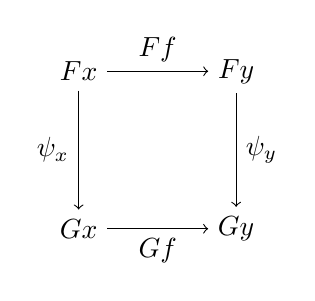
\begin{tikzpicture}
                    \node (FX) at (0, 0) {$Fx$};
                    \node (FY) at(2, 0) {$Fy$};
                    \node (GX) at (0, -2) {$Gx$};
                    \node (GY) at (2, -2) {$Gy$};
                    \draw[->] (FX) -- node[above]{$Ff$} (FY);
                    \draw[->] (GX) -- node[below]{$Gf$} (GY);
                    \draw[->] (FX) -- node[left]{$\psi_x$} (GX);
                    \draw[->] (FY) -- node[right]{$\psi_y$} (GY);
                \end{tikzpicture}
            \end{gather*}
        \end{enumerate}
        It is often said that \textbf{$\psi_x$ is natural in $x$}.
    }
    \begin{notation}
        A natural transformation $\psi$ from a functor $F$ to a functor $G$ is denoted by $\psi:F\Rightarrow G$.\footnote{This is in analogy with the notation for general 2-morphisms. See section \ref{cat:higher_category_theory} for more information.}
    \end{notation}

    \begin{example}[Representation]
        Consider a group $G$ together with its delooping $\mathbf{B}G$ (see definition \ref{cat:group_delooping}). When considering representations as functors $\rho:\mathbf{B}G\rightarrow\mathbf{FinVect}$ we see that the intertwiners\footnote{See definition \ref{group:equivariant}.} are exactly the natural transformations.
    \end{example}

    \newdef{Dinatural transformation}{
        Consider two profunctors $\profunc{F,G}{C}{C}$. A dinatural transformation is a family of morphisms \[\eta_x:F(x, x)\rightarrow G(x, x)\] such that diagram \ref{fig:dinatural} commutes for every morphism $f:y\rightarrow x$.

        \begin{figure}[ht!]
            \centering
            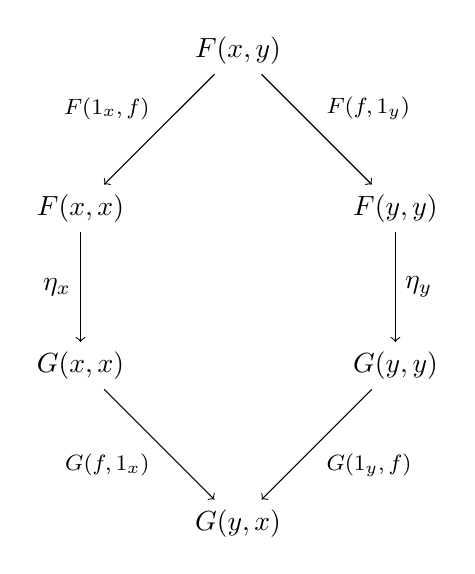
\begin{tikzpicture}
                \node (ab) at (0, 6) {$F(x, y)$};
                \node (F1) at (-2, 4) {$F(x, x)$};
                \node (F2) at (2, 4) {$F(y, y)$};
                \node (G1) at (-2, 2) {$G(x, x)$};
                \node (G2) at (2, 2) {$G(y, y)$};
                \node (ba) at (0, 0) {$G(y, x)$};

                \draw[->] (ab) edge node[above left]{\footnotesize$F(\mathbbm{1}_x, f)$} (F1) (F1) edge node[left]{$\eta_x$} (G1) (G1) edge node[below left]{\footnotesize$G(f, \mathbbm{1}_x)$} (ba);
                \draw[->] (ab) edge node[above right]{\footnotesize$F(f, \mathbbm{1}_y)$} (F2) (F2) edge node[right]{$\eta_y$} (G2) (G2) edge node[below right]{\footnotesize$G(\mathbbm{1}_y, f)$} (ba);
            \end{tikzpicture}
            \caption{Dinatural transformation.}
            \label{fig:dinatural}
        \end{figure}
    }

    \begin{definition}[Functor category]\index{functor!category}
        Let $\mathbf{C}$ be a small category and let $\mathbf{D}$ be a category. The functors $\func{F}{C}{D}$ form the objects of a category with the natural transformations as morphisms. This category is denoted by $\funccat{C}{D}$ or $\mathbf{D}^{\mathbf{C}}$ (analogous to \ref{set:function_set}).
    \end{definition}

    \newdef{Representable functor}{\index{functor!representable}
        Let $\mathbf{C}$ be a locally small category. A functor $\func{F}{C}{Set}$ is said to be representable if there exists an object $x\in\ob{C}$ such that $F$ is naturally isomorphic to $h^x$. The pair $(x,\psi)$, where $\psi$ is the natural isomorphism, is called a \textbf{representation} of $F$.
    }
    \remark{A similar definition exists for contravariant functors $G:\mathbf{C}^{op}\rightarrow\mathbf{Set}$. In this case $\mathbf{C}(x, -)$ has to be replaced by $\mathbf{C}(-, x)$.}

    \begin{theorem}[Yoneda's lemma]\index{Yoneda!lemma}
        Let $\mathbf{C}$ be a locally small category and let $\func{F}{C}{Set}$ be a functor. For every object $x\in\ob{C}$ there exists a natural isomorphism\footnote{Here we use the fact that $\text{Nat}(h^-, -)$ can be seen as a functor $\mathbf{Set}^{\mathbf{C}}\times\mathbf{C}\rightarrow\mathbf{Set}$.} between the set of natural transformations $\text{\emph{Nat}}(h^x, F)$ and $Fx$. The image of a natural transformation $\psi\in\text{\emph{Nat}}(h^x, F)$ is given by $\psi_x(\mathbbm{1}_x)$.
    \end{theorem}
    \remark{For contravariant functors $G:\mathbf{C}^{op}\rightarrow\mathbf{Set}$ one obtains a similar statement after replacing $\mathbf{C}(x, -)$ by $\mathbf{C}(-, x)$.}

    \begin{result}[Yoneda embedding]
        When $F$ is another hom-functor $h^y$ we obtain the following result:
        \begin{gather}
            \text{Nat}(h^x, h^y)\cong\mathbf{C}(y, x)
        \end{gather}
        where one should pay attention to the right-hand side where $y$ appears in the first argument.

        Let $\mathbf{C}(f, -)$ denote the natural transformation corresponding to the morphism $f\in\mathbf{C}(y,x)$. The functor $h^-$ mapping an object $x\in\ob{C}$ to its hom-functor $\mathbf{C}(x, -)$ and a morphism $f\in\mathbf{C}(y, x)$ to the natural transformation $\mathbf{C}(f, -)$ can also be interpreted as a covariant functor $G:\mathbf{C}^{op}\rightarrow\mathbf{Set}^{\mathbf{C}}$. This way we see that Yoneda's lemma gives us a fully faithful functor (i.e. an embedding) $h^-$ from the opposite category $\mathbf{C}^{op}$ to the functor category $\mathbf{Set}^{\mathbf{C}}$.

        As usual all of this can be done for contravariant functors. This gives us an embedding
        \begin{gather}
            \mathcal{Y}:=h_-:\mathbf{C}\hookrightarrow\widehat{\mathbf{C}}
        \end{gather}
        called the Yoneda embedding.
    \end{result}

\subsection{General constructions}

    \newdef{Dagger category\footnotemark}{\index{category!dagger}\index{involution}\label{cat:dagger_category}
        \footnotetext{Also called a \textbf{$\dag$-category}.}
        A category equipped with a contravariant endofunctor, i.e. a functor $\dag:\mathbf{C}^{op}\rightarrow\mathbf{C}$, such that:
        \begin{enumerate}
            \item $\forall c\in\ob{C}: \mathbbm{1}_c^\dag = \mathbbm{1}_c$
            \item $\dag\circ\dag = \mathbbm{1}_c$.
        \end{enumerate}
        The second property says that $\dag$ is an \textbf{involutive} functor.
    }
    \remark{The concept of a dagger structure allows the usual definition of \textbf{unitary} and \textbf{self-adjoint} morphisms.}\index{unitary}
    \begin{property}
        The unitary morphisms in a dagger category form a groupoid\footnote{See definition \ref{cat:groupoid}.}.
    \end{property}

    \newdef{Comma category}{\index{category!comma}
        Let $\mathbf{A}, \mathbf{B}$ and $\mathbf{C}$ be three categories and let $\func{F}{A}{C}$ and $\func{G}{B}{C}$ be two functors. The comma category $F\downarrow G$ is defined as follows:
        \begin{itemize}
            \item Objects are triples $(a, b, \gamma)$ where $a\in\ob{A}, b\in\ob{B}$ and $\gamma:Fa\rightarrow Gb\in\text{hom}(\mathbf{C})$.
            \item Morphisms $(a, b, \gamma)\rightarrow(k, l, \sigma)$ are pairs $(f, g)$ where $f:a\rightarrow k\in\text{hom}(\mathbf{A})$ and $g:b\rightarrow l\in\text{hom}(\mathbf{B})$ such that $\sigma\circ Ff = Gg\circ\gamma$.
            \item Composition of morphisms is defined componentwise.
        \end{itemize}
    }
    \newdef{Slice category}{\index{category!slice}
        Let $\mathbf{C}$ be a category and let $c\in\ob{C}$. The slice category $\mathbf{C}/c$ of $\mathbf{C}$ over $c$ is defined as follows:
        \begin{itemize}
            \item The objects are morphisms in $\mathbf{C}$ with codomain $c$.
            \item The morphisms $f\rightarrow g$ are morphisms $h$ in $\mathbf{C}$ such that $g\circ h = f$.
        \end{itemize}
        This category is also called the \textbf{over-category} of $c$. By dualizing one obtains the \textbf{under-category} of $c$.
    }

\subsection{\difficult{Fibred categories}}

    \newdef{Fibre category}{\index{fibre!category}
        Let $\func{p}{A}{B}$ be a covariant functor. The fibre category over $b\in\ob{B}$ is the subcategory of $\textbf{A}$ consisting of all objects $a\in\ob{A}$ such that $p(a)=b$ and all morphisms $m:a\rightarrow a'$ such that $p(m)=\mathbbm{1}_b$. We will denote it by $\textbf{A}_\textbf{b}$.

        We also introduce some more terminology: Morphisms in $\mathbf{A}$ which are mapped to a morphism $f$ in $\mathbf{B}$ are called \textbf{$f$-morphisms} and, in particular (using the identification of objects and their identity morphisms), morphisms in $\textbf{A}_\textbf{b}$ are called \textbf{$b$-morphisms}. Similarly, we can define \textbf{$B$-categories} as the categories $\mathbf{A}$ equipped with a (covariant) functor $\func{p}{A}{B}$. It is not hard to see that these form a 2-category under composition of functors that respects the $\mathbf{B}$-category structure.
    }

    \newdef{Cartesian morphism}{\index{Cartesian!morphism}
        Consider a $\mathbf{B}$-category $\func{p}{A}{B}$. A morphism $f$ in $\mathbf{A}$ is called $p$-Cartesian if for every $p(f)$-morphism $\tilde{f}$, with $p(f):b\rightarrow b'$ the projection of $f$ under $p$, there is precisely one $b$-morphism $f_b$ such that $f\circ f_b=\tilde{f}$.
    }
    \sremark{There also exists a notion of \textbf{strong Cartesian morphisms} where one replaces the morphism $\tilde{f}$ by morphisms $\varphi$ and $\nu$ such that $p(\varphi)=p(f)\circ\nu$ and $\nu=p(f_b)$. However, for our case of interest (Grothendieck fibrations) these notions coincide.}

    To clarify the above (technical) definition(s) we can draw the following diagram (where the triangles commute):
    \begin{gather*}
        \begin{tikzpicture}
            \node (X3) at (0,2) {$\forall x'$};
            \node (X1) at (0,0) {$x_1$};
            \node (X2) at (2,0) {$x_2$};
            \node (arrow) at (4,1) {$\overset{p}{\mapsto}$};
            \node (pX3) at (6,2) {$p(x')$};
            \node (pX1) at (6,0) {$p(x_1)$};
            \node (pX2) at (8,0) {$p(x_2)$};
            \draw[->] (X1) -- node[below]{$f$} (X2);
            \draw[->] (X3) -- node[left]{$\exists! f_b$} (X1);
            \draw[->] (X3) -- node[above right]{$\forall\varphi$} (X2);
            \draw[->] (pX1) -- node[below]{$p(f)$} (pX2);
            \draw[->] (pX3) -- node[left]{$\forall \nu$} (pX1);
            \draw[->] (pX3) -- node[above right]{$p(\varphi)$} (pX2);
        \end{tikzpicture}
    \end{gather*}
    The diagram for (weak) Cartesian morphisms is obtained by identifying the objects $p(x')$ and $p(x_1)$ and by restricting to the case $\nu=\mathbbm{1}_{p(x_1)}$.

    The Cartesian morphisms are said to be \textbf{inverse images} of their projections under $p$ and the object $x_1$ is called an \textbf{inverse image} of $x_2$ by $p(f)$. The Cartesian morphisms of a fibre category are exactly the isomorphisms of that category.

    \newdef{Fibred category\footnotemark}{\index{fibred category}\index{Grothendieck!fibration|see{fibred category}}
        \footnotetext{Also called a \textbf{Grothendieck fibration}.}
        A $\mathbf{B}$-category $\func{p}{A}{B}$ is called a fibred ($\mathbf{B}$-)category if each morphism in $\mathbf{B}$ whose codomain lies in the range of $p$ has at least one inverse image (in the weak sense) and if the composition of two Cartesian morphisms is again Cartesian (in the weak sense). If one instead works with strongly Cartesian morphisms then the closure under composition follows from the first part of the definition.
    }
    \newdef{Cleavage}{\index{cleavage}\index{cloven|see{cleavage}}
        Given a $\mathbf{B}$-category $\func{p}{A}{B}$ a cleavage is the choice of a Cartesian morphism $f:a\rightarrow a'$ for every $a\in\ob{A}$ and morphism $g:b\rightarrow p(a')$ such that $p(f)=g$. A $\mathbf{B}$-category equipped with a cleavage is said to be \textbf{cloven}.

        It is clear that thee existence of cleavage is sufficient for a category to be fibred and conversely under the axiom of choice every fibred category admits a cleavage.
    }

    \begin{example}[Discrete fibration]\index{fibration}
        Let $\func{F}{A}{B}$ be a functor. $F$ is a discrete fibration if for every object $A\in\ob{A}$ and every morphism $f:B\rightarrow FA$ in $\mathbf{B}$ there exists a unique morphism $g:C\rightarrow A$ in $\mathbf{A}$ such that $F(g) = f$.
    \end{example}

\subsection{Adjunctions}\label{section:category:adjunction}

    \newdef{Hom-set adjunction}{\index{adjunction}
        Let $\func{F}{C}{D}$ and $\func{G}{D}{C}$ be two functors. These functors form a hom-set adjunction (often just called an adjunction) if the following isomorphism is natural in $a, b$:
        \begin{gather}
            \mathbf{D}(Fa, b)\cong\mathbf{C}(a, Gb).
        \end{gather}
        The functor $F$ (resp. G) is called the left (resp. right) adjoint\footnote{Sometimes the word \textbf{adjunct} is used (French versus Latin).}.
    }
    \begin{notation}
        An adjunction $(F, G)$ between categories $\mathbf{C}, \mathbf{D}$ is often denoted by \[\mathbf{D}\adj{F}{G}\mathbf{C}\] or, if the ambient categories are clear, by \[F\dashv G.\]
    \end{notation}

    \newdef{Unit-counit adjunction}{\index{triangle!identities}\index{unit}\index{zig-zag|see{triangle identity}}
        Let $\func{F}{C}{D}$ and $\func{G}{D}{C}$ be two functors. These functors form a unit-counit adjunction if there exist natural transformations
        \begin{align}
            \varepsilon: F\circ G\Rightarrow 1_D\\
            \eta: 1_C\Rightarrow G\circ F
        \end{align}
        such that the following compositions are identity morphisms:
        \begin{align}
            F\xrightarrow{F\eta}FGF\xrightarrow{\varepsilon F}F\\
            G\xrightarrow{\eta G}GFG\xrightarrow{G\varepsilon}G.
        \end{align}
        These identities are sometimes called the \textbf{triangle identities} or \textbf{zig-zag identities} (the latter results from the shape of the associated string diagram). The transformations $\eta$ and $\varepsilon$ are called the \textbf{unit} and \textbf{counit} respectively.
    }

    \begin{property}
        Every hom-set adjuction induces a unit-counit adjunction. Let $\Phi_{a, b}$ be the natural isomorphism associated to the hom-set adjunction $F\dashv G$. The unit $\varepsilon_d$ is obtained as the adjunct $\Phi^{-1}_{Gd, d}(\mathbbm{1}_{Gd})$ of the identity morphism on $Gd\in\ob{C}$ and the counit $\eta_c$ is analogously defined as the adjunct $\Phi_{c, Fc}(\mathbbm{1}_{Fc})$ of the identity morphism at $Fc\in\ob{D}$.

        Similarly, every unit-counit adjunction induces a hom-set adjunction. Consider a morphism $f:Fc\rightarrow d$. The (right) adjunct $\tilde{f}$ is defined as the composition \[\tilde{f}:=Gf\circ\eta_c:c\rightarrow (G\circ F)c\rightarrow Gd.\] To construct the (left) adjunct $g$ we consider a morphism $\tilde{g}:c\rightarrow Gd$: \[g:=\varepsilon_d\circ F\tilde{g}: Fc\rightarrow (F\circ G)d\rightarrow d.\]
    \end{property}

    Now it should be obvious that the above definition of a unit-counit adjunction can be generalized to general 2-categories\footnote{See section \ref{cat:higher_category_theory} for more information.}:
    \newdef{\difficult{Adjunction in 2-category}}{\index{adjunction}
        Let $\mathbf{C}$ be a 2-category. An adjunction in $\mathbf{C}$ is a pair of 1-morphisms $F:a\rightarrow b$ and $G:b\rightarrow a$ together with 2-morphisms $\varepsilon:F\circ G\Rightarrow\mathbbm{1}_b$ and $\eta:\mathbbm{1}_a\Rightarrow G\circ F$ that satisfy the zig-zag identities.
    }

    \begin{remark}[Duals and adjunctions]
        If one looks at the defining relations of duals in a rigid monoidal category one should see that these are in fact the same as the defining relations of the unit and counit of an adjunction. This is a consequence of the fact that a 2-category with a single object can be regarded as a (strict) monoidal category where the composition in the 2-category becomes the tensor product in the monoidal category. Similarly, adjoint 1-morphisms in the 2-category become duals in the monoidal category.
    \end{remark}

\subsection{Monads}

    \newdef{Monad}{\index{monad}\label{cat:monad}
        A monad is a triple $(T, \mu, \eta)$ where $\func{T}{C}{C}$ is an endofunctor and $\mu:T^2\rightarrow T, \eta:\text{id}_{\mathbf{C}}\rightarrow T$ are natural transformations satisfying the following (coherence) conditions:
        \begin{enumerate}
            \item As natural transformation from $T^3$ to $T$ we have
            \begin{gather}
                \mu\circ T\mu = \mu\circ\mu_T.
            \end{gather}
            \item As natural transformation from $T$ to itself we have
            \begin{gather}
                \mu\circ T\eta = \mu\circ\eta_T = \mathbbm{1}.
            \end{gather}
        \end{enumerate}
        These conditions say that a monad is a monoid in the category $\mathbf{End}_{\mathbf{C}}$ of endofunctors on $\mathbf{C}$. Accordingly we often call $\eta$ and $\mu$ the \textbf{unit} and \textbf{multiplication} maps.
    }

    \begin{example}[Adjunction]
        Every adjunction $F\dashv G$, with unit $\varepsilon$ and counit $\eta$, induces a monad of the form $(GF, G\varepsilon F, \eta)$.
    \end{example}

    \newdef{Algebra\footnotemark\ over a monad}{\index{algebra!over a monad}
        \footnotetext{A more suitable name would be ''module over a monad'', since these are modules over a monoid if we view monads as monoids in $\mathbf{End}_{\mathbf{C}}$.}
        Consider a monad $(T, \mu, \eta)$ on a category $\mathbf{C}$. A algebra over $T$ is a couple $(a, \kappa)$ where $a\in\ob{C}$ and $\kappa:Ta\rightarrow a$ such that the following conditions are satisfied:
        \begin{enumerate}
            \item $\kappa\circ T\kappa = \kappa\circ\mu_a$
            \item $\kappa\circ\eta_a = \mathbbm{1}_a$.
        \end{enumerate}
        Morphisms $(a, \kappa_a)\rightarrow(b, \kappa_b)$ of $T$-algebras are morphisms $f:a\rightarrow b$ in $\mathbf{C}$ such that $f\circ\kappa_a = \kappa_b\circ Tf$. An algebra of the form $(Ta, \mu_a)$ is said to be \textbf{free}.
    }
    \newdef{Eilenberg-Moore category}{\index{Eilenberg-Moore category}
        Given a monad $T$ over a category $\mathbf{C}$ we define the Eilenberg-Moore category $\mathbf{C}^T$ as the category of $T$-algebras.
    }
    \newdef{Kleisli category}{\index{Kleisli category}
        Consider a monad $T$ on a category $\mathbf{C}$. The Kleisli category $\mathbf{C}_T$ is the full subcategory of $\mathbf{C}^T$ on the \textbf{free} $T$-algebras. This is equivalently the category with objects $\text{ob}(\mathbf{C}_T):=\ob{C}$ and morphisms $\mathbf{C}_T(a, b):=\mathbf{C}(a, Tb)$.
    }

    \newdef{Monadic adjunction}{\index{adjunction!monadic}
        An adjunction between categories $\mathbf{C}$ and $\mathbf{D}$ is said to be monadic if there exists an equivalence between $D$ and the Eilenberg-Moore category of the induced monad.
    }
    \newdef{Monadic functor}{\index{functor!monadic}
        A functor is said to be monadic if it admits a left adjoint such that the adjunction is monadic.
    }

    The following theorem characterizes monadic functors (for more information on some of the concepts, see sections \ref{cat:section:diagrams} and \ref{cat:section:morphisms}):
    \begin{theorem}[Beck's monadicity theorem]\index{Beck}
        Consider a functor $\func{F}{C}{D}$. This functor is monadic if and only if the following conditions are satisfied:
        \begin{itemize}
            \item $F$ admits a left adjoint.
            \item $F$ reflects isomorphisms.
            \item $\mathbf{C}$ has all coequalizers of $F$-split parallel pairs\footnote{These are parallel pairs $f,g$ such that the images $Ff, Fg$ under $F$ admit a split coequalizer (see definition \ref{cat:split_coequalizer}).} and $F$ preserves these coequalizers.
        \end{itemize}
    \end{theorem}
    \remark{A sufficient condition for monadicity is obtained by replacing the third condition above by the following weaker statement: ''$\mathbf{C}$ has all coequalizers of reflexive pairs and $F$ preserves these coequalizers.'' This weaker form is called the \textbf{crude monadicity theorem}.}

    \newdef{Closure operator\footnotemark}{\label{cat:closure_operator}\index{closure!operator}\index{modal operator|see{closure operator}}
        \footnotetext{Also called a \textbf{modal operator}.}
        Consider a monad $\func{T}{C}{C}$ with unit and product maps $\eta, \mu$. This monad is called a closure operator if the product map is a natural isomorphism.

        Given a closure operator $\func{T}{C}{C}$, one calls the object $Tx$ the closure of $x\in\ob{C}$. The \textbf{closing map} of an object $x\in\ob{C}$ is defined as the morphism $\eta_x$ and $x$ is said to be $T$\textbf{-closed} exactly if its closing map is an isomorphism.
    }

    \begin{remark}[\difficult{Bicategories}]
        In fact one can define a monad in any bicategory as a 1-morphism $t:c\rightarrow c$ together with two 2-morphisms that satisfy similar conditions as the ones above. The above definition is then just a specific case of this more general definition applied to $\mathbf{Cat}$.

        In this general setting one can then also define a \textbf{module} over a monad. First of all one can regard any object $a\in\ob{C}$ as a functor from the terminal category $1$. One can then replace $1$ by any other category in the ordinary definition to obtain a general algebra (or module) over a given monad. It is this definition that readily generalizes to bicategories, i.e. a module is a 1-morphism $a:b\rightarrow c$ together with a 2-morphism that satisfies the same conditions as for an algebra over a monad in $\mathbf{Cat}$.
    \end{remark}

\section{Initial and terminal objects}

    \newdef{Initial object}{
        An object $\emptyset$ such that for every other object $x$ there exists a unique morphism $\iota_x:\emptyset\rightarrow x$.
    }
    \newdef{Terminal object}{
        An object $1$ such that for every other object $x$ there exists a unique morphism $\tau_x:x\rightarrow 1$.
    }
    \begin{property}
        If an initial (resp. terminal) object exists, then it is unique (possibly up to isomorphism).
    \end{property}
    \newdef{Well-pointed category}{
        A category for which the terminal object is a generator\footnote{See definition \ref{cat:generator}.}.
    }

    \newdef{Zero object}{\index{zero!object}\label{cat:zero_object}
        An object that is both initial and terminal. The zero object is often denoted by $0$.
    }
    \begin{property}[Zero morphism]
        From the definition of the zero object it follows that for any two objects $a,b$ there exists a unique morphism $0_{ab}:a\rightarrow0\rightarrow b$.
    \end{property}
    \newdef{Pointed category}{\index{pointed!category}\label{category:pointed_category}
        A category containing a zero object.
    }

    \newdef{Global element}{\index{global!element}\label{category:global_element}
        Let $\mathbf{C}$ be a category with terminal object $1$. A global element of an object $c\in\ob{C}$ is a morphism $1\rightarrow c$.
    }
    \newdef{Pointed object}{\index{pointed!object}
        An object $c$ equipped with a global element $1\rightarrow c$. (This morphism is sometimes called the \textbf{basepoint}.)
    }

    \begin{remark}
        In the category $\mathbf{Set}$ the elements of a set $S$ are in one-to-one correspondence with the global elements of $S$. Furthermore, one has the important property (axiom) that two functions $f,g:S\rightarrow S'$ coincide if their evaluation at every element $s\in S$ is equal or, equivalently, if the precompositions with global elements coincide.

        However, this way of checking equality can fail in other categories. Consider for example $\mathbf{Grp}$, the category of groups, with its object $0=\{e\}$. The only morphism from this group to any other group $G$ is the one mapping $e$ to the unit in $G$ ($0$ is also an initial object in $\mathbf{Grp}$). It is obvious that precomposition with this morphism tells us nothing about the equality of other morphisms. To recover the technique used in $\mathbf{Set}$ one needs to generalize the notion of ''element'':
    \end{remark}
    \newdef{Generalized element}{\index{shape}
        Let $\mathbf{C}$ be category and consider an object $c\in\ob{C}$. For any object $y\in\ob{C}$ one calls a morphism $y\rightarrow c$ a generalized element of $c$. The morphisms $y\rightarrow x$ are also called \textbf{$y$-elements} in $c$ or elements of \textbf{shape} $y$ in $c$.
    }

\section{Morphisms and diagrams}\label{cat:section:morphisms}
\subsection{Morphisms}

    \newdef{Section}{\index{section}\index{retract}
        A section of a morphism $f:a\rightarrow b$ is a right-inverse, i.e. a morphism $g:b\rightarrow a$ such that $f\circ g=\mathbbm{1}_b$. $f$ itself is called a \textbf{retraction} and $b$ is a \textbf{retract} of $a$.
    }
    \newdef{Monomorphism}{\index{monomorphism}
        Let $\mathbf{C}$ be a category. A morphism $\mu\in\mathbf{C}(a, b)$ is called a monomorphism\footnote{Sometimes just a \textbf{mono} or a \textbf{monic} morphism.} if for every object $c\in\ob{C}$ and every two morphisms $\alpha_1, \alpha_2\in\mathbf{C}(c, a)$ such that $\mu\circ\alpha_1 = \mu\circ\alpha_2$ we can conclude that $\alpha_1=\alpha_2$.
    }
    \newdef{Epimorphism}{\index{epimorphism}
        Let $\mathbf{C}$ be a category. A morphism $\varepsilon\in\mathbf{C}(a, b)$ is called an epimorphism\footnote{Sometimes just an \textbf{epi} or an \textbf{epic} morphism.} if for every object $c\in\ob{C}$ and every two morphisms $\alpha_1, \alpha_2\in\mathbf{C}(b, c)$ such that $\alpha_1\circ\varepsilon = \alpha_2\circ\varepsilon$ we can conclude that $\alpha_1=\alpha_2$.

        This definition is equivalent to stating that the pushout of $\varepsilon$ along itself is the identity.
    }

    \newdef{Split monomorphism}{\index{split}
        A morphism $f:a\rightarrow b$ that is a section of some other morphism $g:b\rightarrow a$. It can be shown that every split mono is in fact a mono and even an \textbf{absolute mono}, i.e. it is preserved by all functors.

        The morphism $g$ can be seen to satisfy the dual condition and hence is called a split epimorphism. Again it can be shown to be an absolute epi.
    }

    \newdef{Balanced category}{\index{category!balanced}\label{category:balanced}
        A category is said to be balanced if every monic epi is an isomorphism.
    }

    \begin{property}[Global elements]
        Every global element\footnote{See definition \ref{category:global_element}.} is monic.
    \end{property}

    \newdef{Reflexive pair}{
        Two parallel morphisms $f,g:a\rightarrow b$ are said to form a reflexive pair if they have a common section, i.e. if there exists a morphism $\sigma:b\rightarrow a$ such that $f\circ\sigma=g\circ\sigma=\mathbbm{1}_b$.
    }

    \newdef{Kernel pair}{\index{kernel}
        Consider a morphism $f:a\rightarrow b$. Its kernel pair is defined as the pullback of $f$ along itself.
    }

    \newdef{Lifts and extensions}{\index{lift}\index{extension}
        A lift of a morphism $f:a\rightarrow b$ along an epi $e:x\rightarrow b$ is a morphism $\tilde{f}:a\rightarrow x$ satisfying $f = e\circ\tilde{f}$. The dual of this definition gives rise to extensions. (One sometimes drops the epi/mono condition in these definitions.)
    }
    \newdef{Lifting property}{\index{orthogonal}\label{cat:lifting_property}
        A morphism $f:a\rightarrow b$ has the left lifting property with respect to a morphism $g:c\rightarrow d$ if for every commutative diagram
        \begin{gather*}
            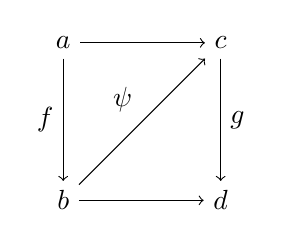
\begin{tikzpicture}
                \node (A) at (0, 0) {$a$};
                \node (B) at (0, -2) {$b$};
                \node (C) at (2, 0) {$c$};
                \node (D) at (2, -2) {$d$};
                \draw[->] (A) -- node[left]{$f$} (B);
                \draw[->] (A) -- (C);
                \draw[->] (B) -- node[above left]{$\psi$} (C);
                \draw[->] (B) -- (D);
                \draw[->] (C) -- node[right]{$g$} (D);
            \end{tikzpicture}
        \end{gather*}
        there exists a morphism $\psi:b\rightarrow c$ such that the triangles commute. The morphism $g$ is also said to have the right lifting property with respect to $f$. If the morphism $\psi$ is unique then $f$ and $g$ are said to be \textbf{orthogonal}.
    }
    \newdef{Injective and projective morphisms}{\index{injective!morphism}\index{projective!morphism}
        Consider a class of morphisms $J\subseteq\text{hom}(\mathbf{C})$. A morphism $f\in\text{hom}(\mathbf{C})$ is said to be $J$-injective (resp. $J$-projective) if it has the right (resp. left) lifting property with respect to all morphisms in $J$.

        Given a set of morphisms $I$ one denotes the set of $I$-injective morphisms by $\text{rlp}(I)$ and the set of $I$-projective morphisms by $\text{llp}(I)$.
    }
    \newdef{Injective and projective objects}{\index{injective!object}\index{projective!object}
        We first give the most abstract definition. If $\mathbf{C}$ has terminal object $\mathbf{1}$, then the we call an object $x$ $J$-injective if the unique morphism $x\rightarrow\mathbf{1}$ is $J$-injective. If $\mathbf{C}$ has an initial object, one can analogously define $J$-projective objects.

        One often modifies this definition by only considering one triangle in the lifting squares:
        \begin{figure}[ht!]
            \centering
            \begin{subfigure}[b]{0.49\textwidth}
                \centering
                \begin{tikzpicture}
                    \node (A) at (0, 0) {$a$};
                    \node (B) at (0, -2) {$b$};
                    \node (C) at (2, 0) {$i$};
                    \draw[->] (A) -- node[left]{$\forall f\in J$} (B);
                    \draw[->] (A) -- node[above]{$g$} (C);
                    \draw[dashed, ->] (B) -- node[below right]{$\exists$} (C);
                \end{tikzpicture}
                \caption{Injective object $i$.}
                \label{fig:injective_object}
            \end{subfigure}
            \begin{subfigure}[b]{0.49\textwidth}
                \centering
                \begin{tikzpicture}
                    \node (A) at (2, 2) {$a$};
                    \node (B) at (2, 0) {$b$};
                    \node (C) at (0, 0) {$p$};
                    \draw[->] (A) -- node[right]{$\forall f\in J$} (B);
                    \draw[->] (C) -- node[below]{$g$} (B);
                    \draw[dashed, ->] (C) -- node[above left]{$\exists$} (A);
                \end{tikzpicture}
                \caption{Projective object $p$.}
                \label{fig:projective_object}
            \end{subfigure}
        \end{figure}

        In general we speak of \textbf{injective} (resp. \textbf{projective}) objects if $J$ is the class of monomorphisms (resp. epimorphisms). For projectives this is equivalent to requiring that the (covariant) hom-functor preserves epimorphisms.

        A category $\mathbf{C}$ is said to \textbf{have enough injectives} if for every object there exists a monomorphism from it into an injective object. The category is said to \textbf{have enough projectives} if for every object there exists an epimorphism from a projective object to it.
    }
    \newdef{Fibrations and cofibrations}{\index{fibration}
        Consider a category $\mathbf{C}$ together with a class $J\subseteq\text{hom}(\mathbf{C})$ of morphisms. A morphism $f\in\text{hom}(\mathbf{C})$ is called a $J$-fibration (resp. $J$-cofibration) if it has the right (resp. left) lifting property with respect to all $J$-projective (resp. $J$-injective) morphisms.
    }

    \newdef{Subobject}{\index{subobject}
        Let $\mathbf{C}$ be a category and let $a\in\ob{C}$ be any object. A subobject $b$ of $a$ is a mono $b\hookrightarrow a$.

        In fact one should work up to isomorphism and accordingly the formal definition goes as follows: A subobject $b$ of $a$ in the category $\mathbf{C}$ is an isomorphism class of monos $i:b\hookrightarrow a$ in the slice category $\mathbf{C}/a$.
    }
    \newdef{Well-powered category}{\index{category!well-powered}
        A category $\mathbf{C}$ is said to be well-powered if for every object $a\in\ob{C}$ the class of subobjects $\text{Sub}(a)$ is small.
    }

    \newdef{Generator\footnotemark}{\index{generator}\label{cat:generator}
        \footnotetext{Also called a \textbf{separator}.}
        Let $\mathbf{C}$ be a category. A collection of objects $\mathcal{O}\subset\ob{C}$ is called a collection of generators for $\mathbf{C}$ if, given any two objects $a,b\in\ob{C}$ and any two parallel morphisms $f,g:a\rightarrow b$, we have that
        \begin{gather}
            f\neq g\implies\exists o\in\mathcal{O}: \exists h\in\mathbf{C}(o, a): f\circ h\neq g\circ h.
        \end{gather}
        This equivalently says that the generalized elements of the objects in $\mathcal{O}$ are sufficient to distinguish all morphisms in $\mathbf{C}$.
    }

    \newdef{Decategorification}{
        Let $\mathbf{C}$ be a (essentially) small category. The set of isomorphism classes of $\mathbf{C}$ is called the decategorification of $\mathbf{C}$. This is given by a functor $\func{Decat}{Cat}{Set}$.\footnote{This can be generalized to higher category theory to go from $n\mathbf{Cat}$ to $(n-1)\mathbf{Cat}$.}
    }

\subsection{Diagrams and universal constructions}\label{cat:section:diagrams}

    \newdef{Diagram}{\index{diagram}
        A diagram in $\mathbf{C}$ with index category $\mathbf{I}$ is a (covariant) functor $\func{D}{I}{C}$.
    }

    \newdef{Cone}{\index{cone}
        Let $\func{D}{I}{C}$ be a diagram. A cone from $a\in\ob{C}$ to $D$ consists of a family of morphisms $\psi_i:a\rightarrow Di, \forall i\in\ob{I}$ such that $\psi_j = Df\circ\psi_i$ for all morphisms $f:i\rightarrow j\in\text{hom}(\mathbf{I})$, as depicted in figure \ref{fig:cone_component}.

        \begin{figure}[ht!]
            \centering
            \begin{subfigure}[b]{0.49\textwidth}
                \centering
                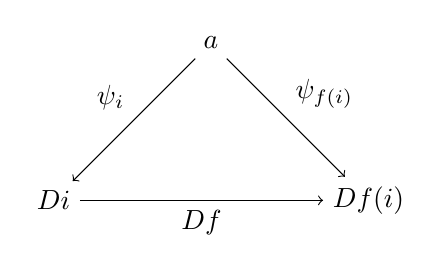
\begin{tikzpicture}
                    \node (1) at (0, 0) {$a$};
                    \node (2) at (-2, -2) {$Di$};
                    \node (3) at (2, -2) {$Df(i)$};
                    \draw[->] (1) -- node[above left]{$\psi_i$} (2);
                    \draw[->] (1) -- node[above right]{$\psi_{f(i)}$} (3);
                    \draw[->] (2) -- node[below]{$Df$} (3);
                \end{tikzpicture}
                \caption{Component of cone over $D$.}
                \label{fig:cone_component}
            \end{subfigure}
            \begin{subfigure}[b]{0.49\textwidth}
                \centering
                \begin{tikzpicture}
                    \node (1) at (0, -2) {$Di$};
                    \node (2) at (-2, 0) {$a$};
                    \node (3) at (2, 0) {$b$};
                    \draw[<-] (1) -- node[below left]{$\psi_i$} (2);
                    \draw[<-] (1) -- node[below right]{$\phi_i$} (3);
                    \draw[->] (2) -- node[above]{$f$} (3);
                \end{tikzpicture}
                \caption{Morphism of cones.}
                \label{fig:cone_morphism}
            \end{subfigure}
            \label{fig:cone}
        \end{figure}
    }
    \begin{adefinition}\index{diagonal!functor}
        This definition can be reformulated by defining an additional functor\footnote{The notation $\Delta_a$ tells us that $\Delta:C\rightarrow [\mathbf{I},\mathbf{C}]$ is the \textbf{diagonal functor}, i.e. $\Delta_c\equiv\Delta(c)$ is the constant functor from $\mathbf{I}$ to $\mathbf{C}$ with target object $c$.} $\Delta_a:\mathbf{I}\rightarrow\mathbf{C}$ that maps every element $i\in\ob{I}$ to $a$ and every morphism $g\in\text{hom}(\mathbf{I})$ to $\mathbbm{1}_a$. The morphisms $\psi_c$ can then be seen as the components of a natural transformation $\psi:\Delta_a\Rightarrow D$. Hence a cone $(a, \psi)$ is an element of $[\mathbf{I}, \mathbf{C}](\Delta_a, D)$.
    \end{adefinition}

    \newdef{Morphism of cones}{\index{morphism!of cones}
        Let $\func{D}{I}{C}$ be a diagram and let $(a, \psi), (b, \phi)$ be two cones to $D$. A morphism between these cones is a morphism of the apexes $f:a\rightarrow b$ such that the diagrams of the form \ref{fig:cone_morphism} commute for all $i\in\ob{I}$. The cones to $D$ together with these morphisms form a category $\mathbf{Cone}(D)$, in fact this can easily be seen to be the comma category $(\Delta \downarrow D)$.
    }
    \newdef{Filtered category}{\index{category!filtered}
        A category in which every finite diagram admits a cocone. For regular cardinals $\kappa$ one can generalize this notion: A  category is said to be $\kappa$-filtered if every diagram with less than $\kappa$ arrows admits a cocone.
    }

    \newdef{Limit}{\index{limit}
        Consider a diagram $\func{D}{I}{C}$. The limit $\lim D$ of this diagram, if it exists, is the terminal object of the category $\mathbf{Cone}(D)$.
    }
    This definition gives us the following universal property:
    \begin{uproperty}\label{cat:limit_uproperty}
        Let $\func{D}{I}{C}$ be a diagram and denote its limit by $\lim D$. For every cone $(c, \psi)\in\mathbf{Cone}(D)$ there exists a unique morphism $f:c\rightarrow\lim D$. This defines a bijection \[[\mathbf{I}, \mathbf{C}](\Delta_c, D) \cong \mathbf{C}(c, \lim D).\]
        If all (small) limits exist then we can define the limit functor $\func{\lim}{[I, C]}{C}$. The universal property of limits then implies that it is right adjoint to the constant functor $\Delta$.
    \end{uproperty}
    \begin{remark}
        In section \ref{section:enriched_category_theory} on enriched category theory we will give a generalization (the so-called \textit{weighted limits}) of the above construction that is better suited to the enriched setting and allows us to express more constructions as (weighted) limits.
    \end{remark}

    \begin{example}[Terminal object]
        The terminal object $1$ is the limit over the empty diagram.
    \end{example}

    \newdef{Finitely complete category}{\index{category!complete}
        A category is said to be finitely complete if it has all finite limits. If all (small) limits exist then the category is said to be \textbf{complete}. The dual notion for colimits is called \textbf{(finite) cocompleteness}.
    }
    \begin{example}[Presheaf categories]\label{cat:complete_presheaf_category}
        All presheaf categories are both complete and cocomplete.
    \end{example}

    \newdef{Continuous functor}{\index{continuity!functor}\label{cat:continuity}
        A functor that preserves all small limits.
    }
    \begin{property}
        In a locally small category every hom-functor is continuous\footnote{They even preserve limits that are not necessarily small.}.
    \end{property}

    In the case where $\mathbf{C}$ is small one can characterize the Yoneda embedding through a universal property:
    \begin{uproperty}[Free cocompletion]\index{cocompletion}\label{cat:free_cocompletion}
        The Yoneda embedding $\mathbf{C}\hookrightarrow\widehat{\mathbf{C}}$ turns the presheaf category $\widehat{\mathbf{C}}$ into the \textbf{free cocompletion} of $\mathbf{C}$, i.e. there exists an equivalence of categories between the functor category of cocontinuous functors $[\widehat{\mathbf{C}}, \mathbf{D}]_{\text{cont}}$ and the ordinary functor category $[\mathbf{C}, \mathbf{D}]$.
    \end{uproperty}

    \newdef{Tiny object}{\index{tiny}
        An object in a locally small category such that its covariant hom-functor preserves small colimits. This is sometimes called a \textbf{small-projective} object since it is in particular projective (epimorphisms are characterized by a pushout).
    }
    \newdef{Cauchy completion}{\index{Cauchy!completion}
        Let $\mathbf{C}$ be a small category. An important (small and full) subcategory of the free cocompletion of $\mathbf{C}$, i.e. the presheaf category $\mathbf{Psh}(\mathbf{C})$, is given by the subcategory of tiny objects. It can be shown that the free cocompletion of the Cauchy completion coincides with the one on $\mathbf{C}$ (up to equivalence).

        A category is said to be \textbf{Cauchy-complete} if it is equivalent to its Cauchy completion. It can be shown that a category is Cauchy-complete if and only if it has all small absolute colimits.
    }

    \newdef{Directed limit}{\index{limit!directed}
        Consider a diagram $\func{D}{I}{C}$. The limit (resp. colimit) of $D$ is said to be codirected (resp. directed) if $\mathbf{I}$ is a downward (resp. upward) directed set\footnote{See definition \ref{set:directed_set}.}.
    }
    The following definition is a categorification of the previous one:
    \newdef{Filtered limit}{\index{limit!filtered}
        Consider a diagram $\func{D}{I}{C}$. The limit (resp. colimit) of $D$ is said to be cofiltered (resp. filtered) if $\mathbf{I}$ is a cofiltered (resp. filtered) category.
    }
    \begin{property}\label{cat:directed_filtered}
        A category has all directed colimits if and only if it has all filtered colimits. (A dual statement holds for limits.)
    \end{property}
    \newdef{Compact object}{\index{compact}\index{presentable}
        An object for which the covariant hom-functor preserves all filtered colimits. These objects are also said to be \textbf{finitely presentable}.\footnote{This name derives from the fact that modules are finitely presented if and only if their covariant hom-functor preserves direct limits (i.e. directed colimits in the context of algebra).}
    }

    \newdef{Product}{\index{product}\index{coproduct}
        Let $\mathbf{I}$ be a discrete category. The (co)limit over a diagram $\func{D}{I}{C}$ is called a (co)product in $\mathbf{C}$.
    }

    \newdef{Equalizer}{\index{equalizer}\index{fork}
        Consider the following diagram:\[x\overset{f}{\underset{g}{\rightrightarrows}} y.\] The limit of this diagram is called the equalizer of $f$ and $g$. Explicitly the equalizer is the universal object $e$ together with a morphism $\varepsilon: e\rightarrow x$ such that the following \textbf{fork} diagram
        \begin{gather}
            e\xrightarrow{\varepsilon}x\overset{f}{\underset{g}{\rightrightarrows}} y
        \end{gather}
        is universal with respect to $(e, \varepsilon)$. By dualizing one obtains \textbf{cofork} diagrams $x\rightrightarrows y\rightarrow z$ and their universal versions, the \textbf{coequalizers}.
    }
    \newdef{Split coequalizer}{\index{split}\label{cat:split_coequalizer}
        A cofork together with a section $\varphi$ of $f$ and a section $\sigma$ of $t$ such that $\sigma\circ t = g\circ \varphi$.
    }

    \newdef{Regular monomorphism}{\index{regular!morphism}
        A mono is said to be regular if it arises as an equalizer of two parallel morphisms. Dually one says that an epi is regular if it arises as a coequalizer.
    }
    \begin{property}[Regular bimorphism]\label{category:regular_iso}
        Both monic regular epimorphisms and epic regular monomorphisms are isomorphisms.
    \end{property}

    \newadef{Finitely complete category}{
        A category is said to be finitely complete if it has a terminal object and if all binary equalizers and products exist.
    }

    \newdef{Span}{\index{span}
        A span in a category $C$ is a diagram of the form \ref{fig:cat_span}.

        Let $\mathbf{\Lambda}$ be the category with three objects $\{-1, 0, 1\}$ and two morphisms $i:0\rightarrow -1$ and $j:0\rightarrow 1$. By the above definition of a diagram a span in $C$ is equivalent to a functor $\func{S}{\Lambda}{C}$.
    }

    \newdef{Pullback\footnotemark}{\index{pullback}\label{cat:pullback}
        \footnotetext{Also called a \textbf{fibre product} or \textbf{Cartesian square}.}
        The pullback of two morphisms $f:a\rightarrow c$ and $g:b\rightarrow c$ is defined as the limit of cospan \ref{fig:pullback}.

        \begin{figure}[!ht]
            \centering
            \begin{subfigure}[b]{0.49\textwidth}
                \centering
                \begin{tikzpicture}
                    \node (A) at (-2, 0) {$a$};
                    \node (S) at (0, 2) {$s$};
                    \node (B) at (2, 0) {$b$};
                    \draw[->] (S) -- node[above left]{$f$} (A);
                    \draw[->] (S) -- node[above right]{$g$} (B);
                \end{tikzpicture}
                \caption{Span (category theory).}
                \label{fig:cat_span}
            \end{subfigure}
            \begin{subfigure}[b]{0.49\textwidth}
                \centering
                \begin{tikzpicture}
                    \node (A) at (-2, 2) {$a$};
                    \node (S) at (0, 0) {$c$};
                    \node (B) at (2, 2) {$b$};
                    \draw[<-] (S) -- node[below left]{$f$} (A);
                    \draw[<-] (S) -- node[below right]{$g$} (B);
                \end{tikzpicture}
                \caption{Cospan.}
                \label{fig:pullback}
            \end{subfigure}
            \caption{}
        \end{figure}
    }

    \begin{notation}[Pullback]
        The pullback of two morphisms $f:a\rightarrow c$ and $g:b\rightarrow c$ is often denoted by $a\times_c b$.
    \end{notation}

    \begin{property}
        If a terminal object $\mathbf{1}$ exists, the pullback $a\times_{\mathbf{1}}b$ is equal to the (Cartesian) product $a\times b$.
    \end{property}
    \newdef{Pushout}{\index{pushout}
        The dual notion of a pullback, i.e. the colimit of a span.
    }

    \begin{property}
        Pullbacks preserve monos. Dually, pushouts preserve epis.
    \end{property}

    \begin{property}[Span category]\label{cat:span_category}
        Consider a category $\mathbf{C}$ with pullbacks. The category $\mathbf{Span}(\mathbf{C})$ is defined as the category with the same objects as $\mathbf{C}$ but with spans as morphisms. Composition of spans is given by pullbacks. By including morphisms of spans, one can refine $\mathbf{Span}(\mathbf{C})$ to a bicategory.
    \end{property}

    \newdef{Wedge}{\index{wedge}
        Consider a profunctor $\profunc{F}{C}{C}$. A wedge $e:w\rightarrow F$ is an object $w\in\ob{Set}$ together with a collection of morphisms $e_c:w\rightarrow F(c, c)$ indexed by $\ob{C}$ such that for any morphism $f:c\rightarrow c'$ the following diagram commutes:
        \begin{gather*}
            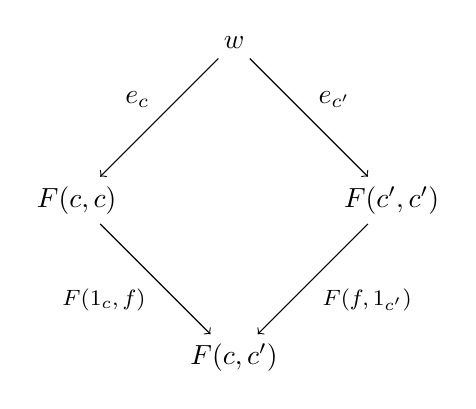
\begin{tikzpicture}
                \node (W) at (0, 4) {$w$};
                \node (F1) at (-2, 2) {$F(c, c)$};
                \node (F2) at (2, 2) {$F(c', c')$};
                \node (F) at (0, 0) {$F(c, c')$};
                \draw[->] (W) edge node[above left]{$e_c$} (F1) (F1) edge node[below left]{\footnotesize$F(\mathbbm{1}_c, f)$} (F);
                \draw[->] (W) edge node[above right]{$e_{c'}$} (F2) (F2) edge node[below right]{\footnotesize$F(f, \mathbbm{1}_{c'})$} (F);
            \end{tikzpicture}
        \end{gather*}
        As was the case for cones, one can reformulate this in terms of (di)natural transformations. A wedge $(w, e)$ of a profunctor $\profunc{F}{C}{C}$ is a dinatural transformation from the constant profunctor $\Delta_w$ to $F$.
    }
    \newdef{End}{\index{end}
        The end of a profunctor $\profunc{F}{C}{C}$ is defined as the universal wedge of $F$. The components of the wedge are called the \textbf{projection maps} of the end. This stems from the fact that for a discrete category the end coincides with the product $\prod_{c\in\ob{C}}F(c, c)$.

        This is equivalent to a definition in terms of equalizers. Consider the two canonical maps $\prod_{c\in\ob{C}}\mathbf{C}(c, c)\rightrightarrows\prod_{f:c\rightarrow c'}\mathbf{C}(c, c')$. This diagram can be interpreted as the product of all lower halves of the wedge diagrams above. It is not hard to see that its equalizer then (universally) satisfies the wedge condition for all $f\in\text{hom}(\mathbf{C})$.
    }
    \newnot{End}{
        The end of a profunctor $\profunc{F}{C}{C}$ is often denoted using an integral sign with subscript: \[\int_{c\in\mathbf{C}}F(c, c).\] For the dual construction, i.e. a \textbf{coend}, one uses the integral sign with superscript.
    }
    \begin{example}[Natural transformations]
        Consider two functors $\func{F, G}{C}{D}$. The map $(c, c')\mapsto\mathbf{D}(Fc, Gc')$ gives a profunctor $\profunc{H}{C}{C}$. If we look at the wedge condition for this profunctor (especially the lower half) we get the following equality for all morphisms $f:c\rightarrow c'$:
        \begin{gather}
            \tau_{c'}\circ Ff = Gf\circ \tau_c
        \end{gather}
        where $\tau_c$ is the projection of the wedge associated to the object $c\in\ob{C}$. Comparing this equality to definition \ref{cat:natural} we immediately see that
        \begin{gather}
            \label{cat:natural_end}
            \text{Nat}(F, G) = \int_{c\in\mathbf{C}}\mathbf{D}(Fc, Gc).
        \end{gather}
    \end{example}

    \begin{property}
        Using the continuity\footnote{See definition \ref{cat:continuity}.} of the hom-functor one can prove the following equality which can be used to turn ends into coends and vice versa:
        \begin{gather}
            \mathbf{Set}\left(\int^{c\in\mathbf{C}}F(c, c), c'\right) = \int_{c\in\mathbf{C}}\mathbf{Set}\left(F(c, c), c'\right).
        \end{gather}
    \end{property}

    Using the above properties and definitions one obtains the following two statements, called the \textbf{Yoneda reduction} and \textbf{co-Yoneda lemma}:
    \begin{theorem}[Ninja Yoneda lemma]\index{Yoneda!lemma}\label{cat:ninja_yoneda}
        Let $\func{F}{C}{D}$ be a covariant functor. The following two isomorphisms follow from the ordinary Yoneda lemma (and the above property):
        \begin{gather}
            \int_{c\in\mathbf{C}}\mathbf{Set}\left(\mathbf{C}(-, c), Fc\right)\cong F
        \end{gather}
        \begin{gather}
            \int^{c\in\mathbf{C}}\mathbf{C}(c, -)\times Fc\cong F.
        \end{gather}
        \emph{For a generalization to the enriched setting see definition \ref{cat:enriched_kan_extension}.}
    \end{theorem}
    \begin{remark}
        A common remark at this point is the comparison with the Dirac distribution \ref{distribution:sieving_dirac_delta}:
        \begin{gather}
            \int \delta(x-y)f(x) = f(y).
        \end{gather}
        By interpreting the functor $F$ as a function, we see that the representable functors behave as Dirac distributions.
    \end{remark}

    \newdef{Kan extension}{\index{Kan!extension}\label{cat:kan_extension}
        Consider two functors $\func{F}{C}{D}$ and $\func{G}{C}{E}$. The right Kan extension\footnote{The left Kan extension Lan$_GF$ is obtained by dualizing this construction (flipping the direction of the natural transformation).} of $F$ along $G$ is given by the universal functor $\func{\text{Ran}_GF}{E}{D}$ and natural transformation $\eta:\text{Ran}_GF\circ G\Rightarrow F$:
        \begin{gather*}
            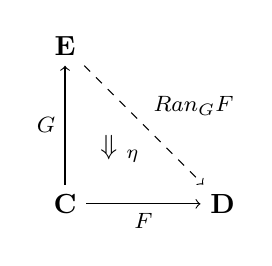
\begin{tikzpicture}
                \node (E) at (0, 2) {$\mathbf{E}$};
                \node (C) at (0, 0) {$\mathbf{C}$};
                \node (D) at (2, 0) {$\mathbf{D}$};
                \node (A) at (0.7, 0.7) {$\Downarrow_{\ \eta}$};
                \draw[->] (C) -- node[left]{\footnotesize$G$} (E);
                \draw[->] (C) -- node[below]{\footnotesize$F$} (D);
                \draw[dashed, ->] (E) -- node[above right]{\footnotesize$\text{Ran}_GF$} (D);
            \end{tikzpicture}
        \end{gather*}
        Universality means that every other natural transformation $\chi:H\circ G\Rightarrow F$ factors uniquely through $\eta$.
    }

    \begin{property}
        Complete (resp. cocomplete) categories admit all right (resp. left) Kan extensions.
    \end{property}

    \newdef{Absolute Kan extension}{
        A (left) Kan extension $\text{Lan}_GF$ is said to be absolute if for every functor $H$ with the same codomain as $F$ the following isomorphism holds:
        \begin{gather}
            H(\text{Lan}_GF)\cong\text{Lan}_G(HF).
        \end{gather}
        There exists an analogous definition for right Kan extensions.
    }
    \newdef{Pointwise Kan extension}{\label{cat:pointwise_kan_extension}
        A Kan extension is said to be pointwise if it is preserved by all representable functors.
    }

    \newadef{Kan extension}{\index{Kan!extension}
        The construction above gives a functor $\text{Ran}_G$ from the functor category $\funccat{C}{D}$ to the functor category $\funccat{E}{D}$. The right Kan extension $\text{Ran}_G$ can be defined as the right adjoint to the pullback functor $G^*:F\mapsto F\circ G$. Similarly one can define the left Kan extension as the left adjoint to the pullback functor $G^*$.

        In the spirit of partial adjoints we can use this definition to define \textbf{local Kan extensions}. Although the left (or right) Kan extension functors do not have to exists globally, the extension of a single functor could still exist. This local version is defined by the following natural isomorphism (here given for a left extension):
        \begin{gather}
            \funccat{C}{D}(F, G^*-) \cong \funccat{E}{D}(\text{Lan}_GF, -).
        \end{gather}
    }
    \remark{Using this equivalence of hom-spaces one can generalize the Kan extension from $\mathbf{Cat}$ to any 2-category.}

    \begin{example}[Limit]
        Denote the terminal category by $\mathbf{1}$. By choosing the functor $G$ in the definition of a right Kan extension to be the unique functor $!_C:\mathbf{C}\rightarrow\mathbf{1}$ into the terminal category one obtains the universal property characterizing limits \ref{cat:limit_uproperty}. We conclude that $\lim F \cong \text{Ran}_{!_C}F$. Similarly one can obtain the colimit as the left Kan extension.
    \end{example}

    The existence of Kan extensions can also be used to determine the existence of adjoints:
    \begin{property}[Adjoint functors]
        A functor $\func{F}{C}{D}$ admits a left adjoint\footnote{An analogous statement holds for right adjoints.} if and only if the right Kan extension of the identity functor $\func{\mathbbm{1}}{C}{C}$ along $F$ exists. If it exists and if it is an absolute extension then the left adjoint is given exactly by this Kan extension.
    \end{property}

    \newdef{Codensity monad}{\index{monad!codensity}\index{codense}
        Consider a general functor $\func{F}{C}{D}$. If the right Kan extension $\text{Ran}_FF$ exists, then it defines a monad. Functors for which this monad is the identity are said to be \textbf{codense}.\footnote{Codense functors are usually defined in a different way, but one can show that this is an equivalent definition (hence the name).} Left Kan extensions give by duality rise to \textit{density comonads}.
    }

\section{Abelian categories}

    \newdef{Pre-additive category}{
        A (locally small) category enriched over $\mathbf{Ab}$, i.e. every hom-set is an Abelian group and composition is bilinear.
    }

    \begin{property}\index{zero!object}
        Let $\mathbf{A}$ be a pre-additive category and consider an object $a\in\ob{A}$. The following statements are equivalent:
        \begin{itemize}
            \item $a$ is an initial object.
            \item $a$ is a final object.
            \item $\mathbbm{1}_a$ = 0.
        \end{itemize}
        It follows that every initial/terminal object in a pre-additive category is automatically is a zero object\footnote{See definition \ref{cat:zero_object}.}.
    \end{property}
    \begin{property}\index{biproduct}
        In a pre-additive category the finite products $\prod_{i\in I}x_i$ are isomorphic to the finite coproducts $\bigsqcup_{i\in I} x_i$ (which are called \textbf{direct sums} in this context). If a product $x\times y$ exists then so does the coproduct $x\sqcup y$ and if the coproduct exists then so does the product. In general if a product and coproduct exist and are equal then one speaks of a \textbf{biproduct}.
    \end{property}

    \newdef{Additive category}{\index{additive!category}
        A pre-additive category in which all finite biproducts exist.
    }

    If one speaks of additive categories, one generally assumes that the associated functors are of a specific type:
    \newdef{Additive functor}{\index{additive!functor}\label{category:additive_functor}
        Let $\mathbf{A}, \mathbf{A'}$ be additive categories. A functor $\func{F}{A}{A'}$ is said to be additive if it preserves finite biproducts, i.e.:
        \begin{enumerate}
            \item It preserves zero objects: $F0_{\mathbf{A}} \cong 0_{\mathbf{A}'}$.
            \item There exists a natural isomorphism $F(x\oplus y)\cong Fx\oplus Fy$ for all $x,y\in\ob{A}$.
        \end{enumerate}
        One can generalize this notion to pre-additive categories. A functor between pre-additive categories is said to be additive if it acts as a group morphism on hom-spaces.
    }

    In a pre-additive category one can define the classical notions from (homological) algebra such as images and kernels:
    \newdef{Kernel}{\index{kernel}
        Let $f:x\rightarrow y$ be a morphism. A\footnote{Note the word \textit{a}. The kernel of a morphism is determined up to an isomoprhism.} kernel is a morphism $k:z\rightarrow x$ such that
        \begin{enumerate}
            \item $f\circ k = 0$.
            \item for every other morphism $k':z'\rightarrow x$ such that $f\circ k' = 0$ there exists a unique morphism $h:z'\rightarrow z$ such that $k\circ h = k'$. (This is the universal property characterizing kernels.)
        \end{enumerate}
        Hence a kernel of $f$ is an equalizer of $f$ and 0.
    }
    \begin{notation}[Kernel]
        If the kernel of $f:x\rightarrow y$ exists then it is denoted by $\ker(f)\rightarrow x$.
    \end{notation}

    \newdef{Cokernel}{
        Let $f:x\rightarrow y$ be a morphism. A cokernel is a morphism $p:y\rightarrow z$ such that
        \begin{enumerate}
            \item $p\circ f = 0$.
            \item for every other morphism $p':y\rightarrow z'$ such that $p'\circ f = 0$ there exists a unique morphism $h:z\rightarrow z'$ such that $h\circ p = p'$. (This is the universal property characterizing cokernels.)
        \end{enumerate}
        Hence a cokernel of $f$ is a coequalizer of $f$ and 0.
    }
    \begin{notation}[Cokernel]
        If the cokernel of $f:x\rightarrow y$ exists then it is denoted by $y\rightarrow\text{coker}(f)$.
    \end{notation}
    \remark{The name and notation of the kernel\footnote{Similarly for the cokernel.} (in the categorical sense) is explained by remarking that by Yoneda's lemma the morphism \[\ker(f)\rightarrow x\] represents the functor \[F:z\mapsto\ker\Big(\mathbf{C}(z, x)\rightarrow\mathbf{C}(z, y)\Big).\]}

    \newdef{Pre-Abelian category}{
        An additive category is pre-Abelian if every morphism has a kernel and cokernel.
    }
    \newdef{Abelian category}{\index{Abelian!category}
        A pre-Abelian category in which every mono is a kernel and every epi is a cokernel or equivalently if for every morphism $f$ there exists an isomorphism
        \begin{gather}
            \text{coker}(\ker(f))\cong\ker(\text{coker}(f)).
        \end{gather}
    }

    \begin{property}
        In Abelian categories a morphism is monic if and only if it is injective, i.e. its kernel is 0. Analogously a morphism is epic if and only if it is surjective, i.e. its cokernel is 0.
    \end{property}

    \newdef{$k$-linear category}{\index{category!linear}
        Let $\textbf{Vect}_k$ denote the category of vector spaces over the base field $k$. A $k$-linear category is a category enriched over $\textbf{Vect}_k$. (If the base field is clear, the subscript is often left implicit.)
    }

    \newdef{Exact functor}{\index{exact!functor}
        Let $\func{F}{A}{A'}$ be an additive functor between additive categories. We use the following definitions:
        \begin{itemize}
            \item $F$ is said to be left exact if it preserves kernels.
            \item $F$ is said to be right exact if it preserves cokernels.
            \item $F$ is said to be exact if it is both left and right exact.
        \end{itemize}
    }
    \begin{result}
        The previous definition implies the following properties (which can in fact be used as an alternative definition):
        \begin{itemize}
            \item If $F$ is left exact it maps an exact sequence of the form \[0\longrightarrow a\longrightarrow b\longrightarrow c\]
            to an exact sequence of the form \[0\longrightarrow Fa\longrightarrow Fb\longrightarrow Fc.\]
            \item If $F$ is right exact it maps an exact sequence of the form \[a\longrightarrow b\longrightarrow c\longrightarrow 0\]
            to an exact sequence of the form \[Fa\longrightarrow Fb\longrightarrow Fc\longrightarrow 0.\]
            \item If $F$ is exact it maps short exact sequences to short exact sequences.
        \end{itemize}
    \end{result}

    \begin{theorem}[Freyd-Mitchell embedding theorem]\index{Freyd-Mitchell}\index{embedding!theorem|see{Freyd-Mitchell}}
        Every small Abelian category admits a fully faithful and exact functor into a category of the form $\mathbf{Mod}_R$ for some ring $R$.
    \end{theorem}

\subsection{Finiteness}

    \newdef{Simple object}{\index{simple!object}
        Let $\mathbf{A}$ be an Abelian category. An object $a\in\ob{A}$ is said to be simple if the only subobjects of $a$ are $\mathbf{0}$ and $a$ itself. An object is said to be semisimple if it is a direct sum of simple obejcts.
    }
    \newdef{Semisimple category}{
        A category is said to be semisimple if every object is semisimple (where generally the direct sums are taken over finite index sets).
    }

    \newdef{Jordan-H\"older series}{\index{finite}
        A filtration \[0\rightarrow x_1\rightarrow x_2\rightarrow\cdots\rightarrow x_n=x\] of an object $x$ is said to be a Jordan-H\"older series if the quotient objects $x_i/x_{i-1}$ are simple for all $i\leq n$. If the series is finite, i.e. $n\in\mathbb{N}$, then the object $x$ is said to be \textbf{finite}.
    }
    \begin{theorem}[Jordan-H\"older]\index{Jordan-H\"older}
        If an object $x$ in an Abelian category is finite then every Jordan-H\"older series of $x$ has the same length. In particular, the multiplicities of simple objects are the same for all such series.
    \end{theorem}
    \begin{theorem}[Krull-Schmidt]\index{Krull-Schmidt}\index{indecomposable}
        Any object in an Abelian category of finite length admits a unique decomposition as a direct sum of indecomposable\footnote{An object is \textbf{indecomposable} if it cannot be written as a direct sum of its subobjects.} objects.
    \end{theorem}

    \newdef{Locally finite}{\label{category:locally_finite}
        A $k$-linear Abelian category is said to be locally finite if it satisfies the following conditions:
        \begin{enumerate}
            \item Every hom-space is finite-dimensional.
            \item Every object has finite length.
        \end{enumerate}
    }
    \newdef{Finite}{\index{finite}
        A $k$-linear Abelian category is said to be finite if it satisfies the following conditions:
        \begin{enumerate}
            \item It is locally finite.
            \item It has enough projectives (or equivalently every simple object has a \textit{projective cover}).
            \item The set of isomorphism classes of simple objects is finite.
        \end{enumerate}
    }

    \begin{theorem}[Schur's lemma]\index{Schur's lemma}
        Let $\mathbf{A}$ be an Abelian category. For every two simple objects $x,y$ one has that every nonzero morphism $x\rightarrow y$ is an isomorphism. In particular, if $x,y$ are two non-isomorphic simple objects then $\mathbf{C}(x, y)=0$ and $\mathbf{C}(x, x)$ is a division ring.
    \end{theorem}
    \begin{result}
        If $\mathbf{A}$ is locally finite and $k$ is algebraically closed, then $\mathbf{C}(x, x)\cong k$ for all simple objects $x$. (This follows from the fact that the only finite-dimensional division algebra over an algebraically closed field is itself.)
    \end{result}

    The Freyd-Mitchell theorem can be adapted to the finite linear case as follows:
    \begin{theorem}[Deligne]\index{Deligne}
        Every finite $k$-linear Abelian category is $k$-linearly equivalent to a category of the form $\mathbf{Mod}_A^{\text{fin}}$ for $A$ a finite-dimensional $k$-algebra.
    \end{theorem}

    \begin{construct}[Deligne tensor product]\index{Deligne!tensor product}
        Let $\mathbf{A}, \mathbf{B}$ be two Abelian categories. The Deligne (tensor) product is defined (if it exists) as the category $\mathbf{A}\boxtimes\mathbf{B}$ such that there exists a bijection between right exact functors $\mathbf{A}\boxtimes\mathbf{B}\rightarrow\mathbf{C}$ and right exact functors $\mathbf{A}\times\mathbf{B}\rightarrow\mathbf{C}$ (the latter being right exact in each argument).

        For finite Abelian categories it can be shown that their Deligne product always exists. By the Deligne embedding theorem one can find an explicit description: Consider two finite-dimensional $k$-algebras $A, B$. The category $\mathbf{Mod}_A^{\text{fin}}\boxtimes\mathbf{Mod}_B^{\text{fin}}$ is equivalent to the category of finite-dimensional modules over $A\otimes_kB$.
    \end{construct}

\section{Monoidal categories}

    \newdef{Monoidal category}{\index{monoidal!category}\index{tensor!product}\label{category:monoidal_category}
        A category $\mathbf{C}$ equipped with a bifunctor \[-\otimes -:\mathbf{C}\times\mathbf{C}\rightarrow\mathbf{C}\] called the \textbf{tensor product} or \textbf{monoidal product}, together with a distinct object $\mathbf{1}$, called the \textbf{unit object}, and 3 natural isomorphisms, called the \textbf{coherence maps}:
        \begin{enumerate}
            \item \textbf{Associator}: $\alpha_{a, b, c}:(a\otimes b)\otimes c\cong a\otimes(b\otimes c)$;
            \item \textbf{Left unitor}: $\lambda_a:\mathbf{1}\otimes a\cong a$;
            \item \textbf{Right unitor}: $\rho_a:a\otimes\mathbf{1}\cong a$;
        \end{enumerate}
        such that the \textbf{triangle} and \textbf{pentagon} diagrams commute. (See figures \ref{fig:triangle_diagram} and \ref{fig:pentagon_diagram}.)

        \begin{figure}[ht!]
            \centering
            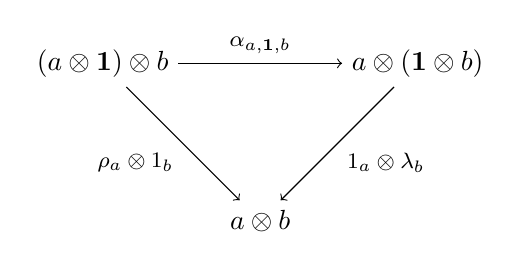
\begin{tikzpicture}
                \node (1) at (0, 0) {$(a\otimes\mathbf{1})\otimes b$};
                \node (2) at (4, 0) {$a\otimes(\mathbf{1}\otimes b)$};
                \node (3) at (2, -2) {$a\otimes b$};
                \draw[->] (1) -- node[above]{\footnotesize$\alpha_{a, \mathbf{1}, b}$} (2);
                \draw[->] (1) -- node[below left]{\footnotesize$\rho_a\otimes\mathbbm{1}_b$} (3);
                \draw[->] (2) -- node[below right]{\footnotesize$\mathbbm{1}_a\otimes\lambda_b$} (3);
            \end{tikzpicture}
            \caption{Triangle diagram.}
            \label{fig:triangle_diagram}
        \end{figure}
        \begin{figure}[ht!]
            \centering
            \begin{tikzpicture}
                \node (1) at (0, 0) {$((a\otimes b)\otimes c)\otimes d$};
                \node (2) at (6, 0) {$(a\otimes (b\otimes c))\otimes d$};
                \node (3) at (-3, -3) {$(a\otimes b)\otimes(c\otimes d)$};
                \node (4) at (9, -3) {$a\otimes((b\otimes c)\otimes d)$};
                \node (5) at (3, -6) {$a\otimes(b\otimes (c\otimes d))$};
                \draw[->] (1) -- node[above]{\footnotesize$\alpha_{a, b, c}\otimes\mathbbm{1}_d$} (2);
                \draw[->] (1) -- node[above left]{\footnotesize$\alpha_{a\otimes b, c, d}$} (3);
                \draw[->] (3) -- node[below left]{\footnotesize$\alpha_{a, b, c\otimes d}$} (5);
                \draw[->] (2) -- node[above right]{\footnotesize$\alpha_{a, b\otimes c, d}$} (4);
                \draw[->] (4) -- node[below right]{\footnotesize$\mathbbm{1}_a\otimes\alpha_{b, c, d}$} (5);
            \end{tikzpicture}
            \caption{Pentagon diagram.}
            \label{fig:pentagon_diagram}
        \end{figure}
    }

    \newdef{Strict monoidal category}{
        A monoidal category for which the associator $\alpha$ and the unitors $\lambda,\rho$ are identity morphisms.
    }

    \newdef{Scalar}{\index{scalar}
        In a monoidal category the scalars are defined as the endomorphisms $\mathbf{1}\rightarrow\mathbf{1}$.
    }
    \begin{property}
        The set of scalars forms a commutative monoid.
    \end{property}
    \begin{property}
        Every scalar $s:\mathbf{1}\rightarrow\mathbf{1}$ induces a natural transformation \[s_a:a\cong\mathbf{1}\otimes a\xrightarrow{s\otimes\mathbbm{1}_a}\mathbf{1}\otimes a\cong a\] satisfying the "usual" rules of scalar multiplication in linear algebra:
        \begin{itemize}
            \item $s\diamond(s'\diamond f) = (s\circ s')\diamond f$
            \item $(s\diamond f)\circ(s'\diamond g) = (s\circ s')\diamond(f\circ g)$
            \item $(s\diamond f)\otimes(s'\diamond g) = (s\circ s')\diamond(f\otimes g)$
        \end{itemize}
        where $s\diamond f$ denotes the composite $f\circ s_a = s_b\circ f$.
    \end{property}

    \newdef{Weak inverse}{\index{weak!inverse}
        Let $(\mathbf{C},\otimes, \mathbf{1})$ be a monoidal category and consider an object $x\in\ob{C}$. An object $y\in\ob{C}$ is called a weak inverse of $x$ if it satisfies $x\otimes y\cong\mathbf{1}$.
    }
    \remark{One can show that the existence of a one-sided weak inverse (as in the definition above) is sufficient to prove that it is in fact a two-sided weak inverse, i.e. $y\otimes x\cong\mathbf{1}$.}

    \begin{theorem}[MacLane's coherence theorem]\index{coherence!theorem}
        Consider two functors $\func{F, G}{C}{D}$ between two monoidal categories $\mathbf{C}, \mathbf{D}$. Any two natural transformations $\eta,\varepsilon:F\Rightarrow G$, constructed solely from the associator $\alpha$ and the unitors $\lambda, \rho$, coincide.
    \end{theorem}

    \newdef{Internal hom}{\index{internal!hom}\label{category:internal_hom}
        Let $(\mathbf{M}, \otimes, \mathbf{1})$ be a monoidal category. In this setting one can generalize the \textit{currying} procedure, i.e. the identification of maps $x\times y\rightarrow z$ with maps $x\rightarrow(y\rightarrow z)$. The ''internal'' hom-functor is defined by the following natural isomorphism:
        \begin{gather}
            \hom(x\otimes y, z)\cong\hom(x, \underline{\hom}(y, z)).
        \end{gather}
        The existence of all internal homs is equivalent to the existence of a right adjoint to the tensor functor.
    }
    \begin{notation}
        The internal hom $\underline{\hom}(a,b)$ is also often denoted by $[a,b]$. From now on we will follow this convention (unless otherwise specified).
    \end{notation}
    \newdef{Closed monoidal category}{\index{closed!category}\index{Cartesian!closed}
        A monoidal category $(\mathbf{C}, \otimes, \mathbf{1})$ is said to be closed monoidal if it has all internal homs. If the monoidal structure is induced by a (Cartesian) product structure, then the category is often called a \textbf{Cartesian closed category}.
    }

    \begin{notation}
        In Cartesian closed categories a different, but frequently used, notation is $a\Rightarrow b$. However, we will not use this as it might confuse with the notation for 2-morphisms.
    \end{notation}
    \begin{property}\label{cat:internal_hom_property}
        The following isomorphism is clearly natural in both $a,b\in\ob{M}$:
        \begin{gather}
            \mathbf{M}(\mathbf{1}, [a,b])\cong\mathbf{M}(a, b).
        \end{gather}
        It is this relation that gives the best explanation for the term ''internal hom''. We also immediately obtain the following natural isomorphism:
        \begin{gather}
            \mathbf{M}(a, [\mathbf{1}, b])\cong\mathbf{M}(a, b)
        \end{gather}
        This implies $[\mathbf{1}, b]\cong b$ because the Yoneda embedding is fully faithful. Although the global elements $\mathbf{M}(\mathbf{1}, b)$ do not fully specify an object $b$, this is still the case internally.
    \end{property}

    \begin{property}[Symmetry]
        Let $M$ be a symmetric monoidal category. The definition of an internal hom can also be internalized, i.e. there exists a natural isomorphism of the form
        \begin{gather}
            [a\otimes b, c]\cong[a, [b, c]].
        \end{gather}
        Furthermore, if $\mathbf{M}$ is also symmetric (see definition \ref{cat:symmetric}) then there exists an internal isomorphism of the form
        \begin{gather}
            \label{cat:internal_symmetry}
            [a, [b, c]]\cong[b, [a, c]].
        \end{gather}
    \end{property}

\subsection{Braided categories}

    \newdef{Braided monoidal category}{\index{braiding}
        Let $(\mathbf{C}, \otimes, \mathbf{1})$ be a monoidal category. $\mathbf{C}$ is called a braided monoidal category if it comes equipped with a natural isomorphism \[\sigma_{a, b}:a\otimes b\cong b\otimes a\]
        such that the two \textbf{hexagon} diagrams in figures \ref{fig:hexagon_diagrams1} and \ref{fig:hexagon_diagrams2} commute. The isomorphism $\sigma$ is called the \textbf{braiding} (morphism).
        \begin{figure}[ht!]
            \centering
            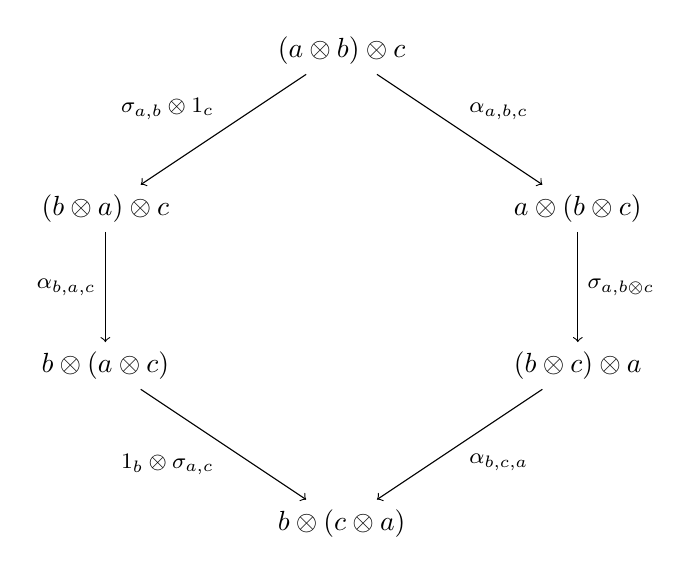
\begin{tikzpicture}
                \node (1) at (0, 0) {$(a\otimes b)\otimes c$};
                \node (2) at (-3, -2) {$(b\otimes a)\otimes c$};
                \node (3) at (3, -2) {$a\otimes(b\otimes c)$};
                \node (4) at (-3, -4) {$b\otimes (a\otimes c)$};
                \node (5) at (3, -4) {$(b\otimes c)\otimes a$};
                \node (6) at (0, -6) {$b\otimes(c\otimes a)$};
                \draw[->] (1) -- node[above left]{\footnotesize$\sigma_{a, b}\otimes\mathbbm{1}_c$} (2);
                \draw[->] (1) -- node[above right]{\footnotesize$\alpha_{a, b, c}$} (3);
                \draw[->] (2) -- node[left]{\footnotesize$\alpha_{b, a, c}$} (4);
                \draw[->] (3) -- node[right]{\footnotesize$\sigma_{a, b\otimes c}$} (5);
                \draw[->] (4) -- node[below left]{\footnotesize$\mathbbm{1}_b\otimes\sigma_{a, c}$} (6);
                \draw[->] (5) -- node[below right]{\footnotesize$\alpha_{b, c, a}$} (6);
            \end{tikzpicture}
            \caption{Hexagon diagram 1.}
            \label{fig:hexagon_diagrams1}
        \end{figure}
        \begin{figure}[ht!]
            \centering
            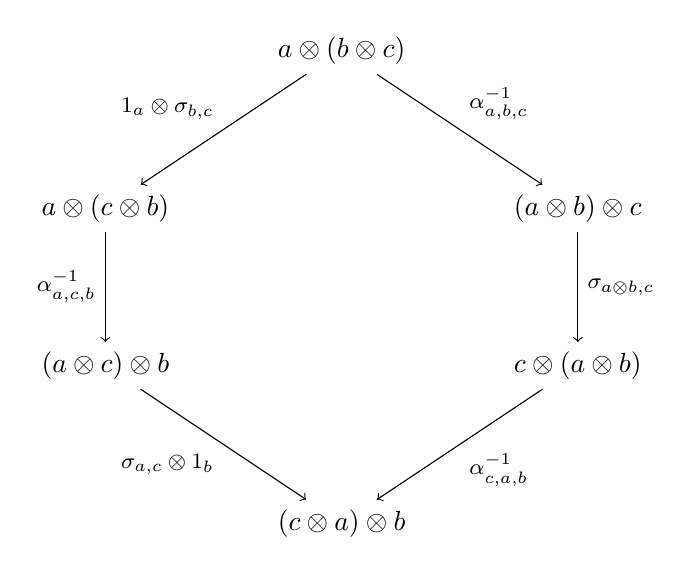
\begin{tikzpicture}
                \node (1) at (0, 0) {$a\otimes(b\otimes c)$};
                \node (2) at (-3, -2) {$a\otimes(c\otimes b)$};
                \node (3) at (3, -2) {$(a\otimes b)\otimes c$};
                \node (4) at (-3, -4) {$(a\otimes c)\otimes b$};
                \node (5) at (3, -4) {$c\otimes(a\otimes b)$};
                \node (6) at (0, -6) {$(c\otimes a)\otimes b$};
                \draw[->] (1) -- node[above left]{\footnotesize$\mathbbm{1}_a\otimes\sigma_{b, c}$} (2);
                \draw[->] (1) -- node[above right]{\footnotesize$\alpha^{-1}_{a, b, c}$} (3);
                \draw[->] (2) -- node[left]{\footnotesize$\alpha^{-1}_{a, c, b}$} (4);
                \draw[->] (3) -- node[right]{\footnotesize$\sigma_{a\otimes b, c}$} (5);
                \draw[->] (4) -- node[below left]{\footnotesize$\sigma_{a, c}\otimes\mathbbm{1}_b$} (6);
                \draw[->] (5) -- node[below right]{\footnotesize$\alpha^{-1}_{c, a, b}$} (6);
            \end{tikzpicture}
            \caption{Hexagon diagram 2.}
            \label{fig:hexagon_diagrams2}
        \end{figure}
    }
    \begin{property}\index{Yang-Baxter}
        The braiding $\sigma_{a,a}$ satisfies the \textit{Yang-Baxter} equation. More generally the braiding $\sigma$ satisfies the following equation for all objects $a,b,c\in\ob{C}$:
        \begin{gather}
            (\sigma_{b,c}\otimes\mathbbm{1}_a)\circ(\mathbbm{1}_b\otimes\sigma_{a,c})\circ(\sigma_{a,b}\otimes\mathbbm{1}_c) = (\mathbbm{1}_c\otimes\sigma_{a,b})\circ(\sigma_{a,c}\otimes\mathbbm{1}_b)\circ(\mathbbm{1}_a\otimes\sigma_{b,c}).
        \end{gather}
    \end{property}
    \remark{When drawing the above equality using string diagrams one sees that the Yang-Baxter equation is equal to the invariance of string diagrams under a \textit{Reidemeister III move}.}

    \newdef{Symmetric monoidal category}{\label{cat:symmetric}
        A braided monoidal category where the braiding $\sigma$ satisfies
        \begin{gather}
            \sigma_{x, y} \circ \sigma_{y, x} = \mathbbm{1}_{x\otimes y}.
        \end{gather}
    }

    In chapter \ref{chapter:hda} the theory of monoidal categories is continued.

\subsection{Monoidal functors}

    \newdef{Monoidal functor}{\index{monoidal!functor}\index{coherence!maps}
        Let $(\mathbf{C}, \otimes, \mathbf{1}_C), (\mathbf{D}, \circledast, \mathbf{1}_D)$ be two monoidal categories. A functor $\func{F}{C}{D}$ is said to be monoidal if there exists:
        \begin{enumerate}
            \item A natural isomorphism $\psi_{a, b}: Fa\circledast Fb\Rightarrow F(a\otimes b)$ such that the diagram in figure \ref{fig:monoidal_functor1} commutes.
                \begin{figure}[ht!]
                    \centering
                    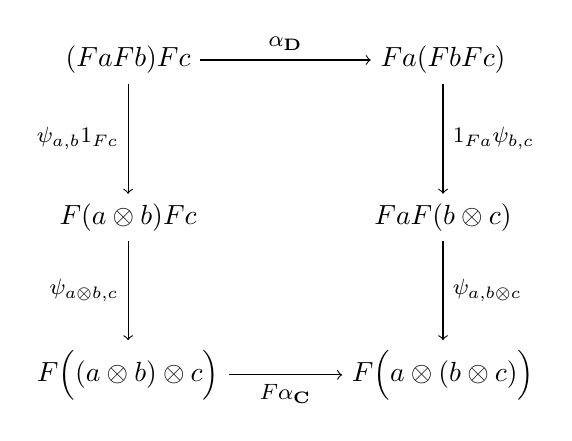
\begin{tikzpicture}
                        \node (1) at (0, 0) {$(Fa\circledast Fb)\circledast Fc$};
                        \node (2) at (4, 0) {$Fa\circledast(Fb\circledast Fc)$};
                        \node (3) at (0, -2) {$F(a\otimes b)\circledast Fc$};
                        \node (4) at (4, -2) {$Fa\circledast F(b\otimes c)$};
                        \node (5) at (0, -4) {$F\Big((a\otimes b)\otimes c\Big)$};
                        \node (6) at (4, -4) {$F\Big(a\otimes (b\otimes c)\Big)$};
                        \draw[->] (1) -- node[above]{\footnotesize$\alpha_{\mathbf{D}}$} (2);
                        \draw[->] (5) -- node[below]{\footnotesize$F\alpha_{\mathbf{C}}$} (6);
                        \draw[->] (1) -- node[left]{\footnotesize$\psi_{a, b}\circledast\mathbbm{1}_{Fc}$} (3);
                        \draw[->] (3) -- node[left]{\footnotesize$\psi_{a\otimes b, c}$} (5);
                        \draw[->] (2) -- node[right]{\footnotesize$\mathbbm{1}_{Fa}\circledast\psi_{b, c}$} (4);
                        \draw[->] (4) -- node[right]{\footnotesize$\psi_{a, b\otimes c}$} (6);
                    \end{tikzpicture}
                    \caption{Monoidal functor.}
                    \label{fig:monoidal_functor1}
                \end{figure}

            \item An isomorphism $\phi: \mathbf{1}_D\rightarrow F\mathbf{1}_C$ which makes the two diagrams in figure \ref{fig:unitality} commute.
            \begin{figure}[ht!]
                \centering
                \begin{subfigure}[b]{0.49\textwidth}
                    \centering
                    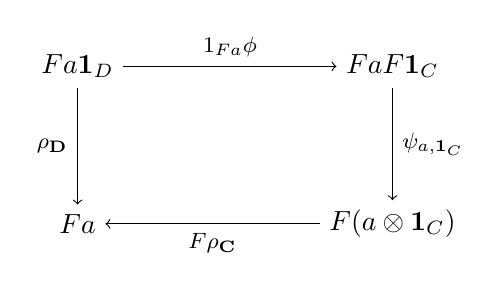
\begin{tikzpicture}
                        \node (1) at (0, 0) {$Fa\circledast\mathbf{1}_D$};
                        \node (2) at (4, 0) {$Fa\circledast F\mathbf{1}_C$};
                        \node (3) at (0, -2) {$Fa$};
                        \node (4) at (4, -2) {$F(a\otimes\mathbf{1}_C)$};
                        \draw[->] (1) -- node[above]{\footnotesize$\mathbbm{1}_{Fa}\circledast\phi$} (2);
                        \draw[<-] (3) -- node[below]{\footnotesize$F\rho_{\mathbf{C}}$} (4);
                        \draw[->] (1) -- node[left]{\footnotesize$\rho_{\mathbf{D}}$} (3);
                        \draw[->] (2) -- node[right]{\footnotesize$\psi_{a, \mathbf{1}_C}$} (4);
                    \end{tikzpicture}
                \end{subfigure}
                \begin{subfigure}[b]{0.49\textwidth}
                    \centering
                    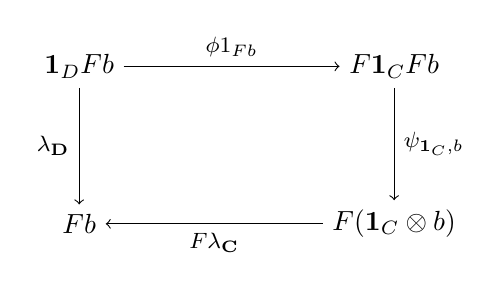
\begin{tikzpicture}
                        \node (1) at (0, 0) {$\mathbf{1}_D\circledast Fb$};
                        \node (2) at (4, 0) {$F\mathbf{1}_C\circledast Fb$};
                        \node (3) at (0, -2) {$Fb$};
                        \node (4) at (4, -2) {$F(\mathbf{1}_C\otimes b)$};
                        \draw[->] (1) -- node[above]{\footnotesize$\phi\circledast\mathbbm{1}_{Fb}$} (2);
                        \draw[<-] (3) -- node[below]{\footnotesize$F\lambda_{\mathbf{C}}$} (4);
                        \draw[->] (1) -- node[left]{\footnotesize$\lambda_{\mathbf{D}}$} (3);
                        \draw[->] (2) -- node[right]{\footnotesize$\psi_{\mathbf{1}_C, b}$} (4);
                    \end{tikzpicture}
                \end{subfigure}
                \caption{Unitality diagrams.}
                \label{fig:unitality}
            \end{figure}
        \end{enumerate}
    }
    \remark{The morphisms $\psi_{a, b}$ and $\phi$ are also called \textbf{coherence maps} or \textbf{structure morphisms}.}

    \begin{property}
        For every monoidal functor $F$ there exists a canonical isomorphism $\phi:\mathbf{1}_D\rightarrow F\mathbf{1}_C$ defined by the commutative diagram in figure \ref{fig:canonical_monoidal_isom}.
        \begin{figure}[ht!]
            \centering
            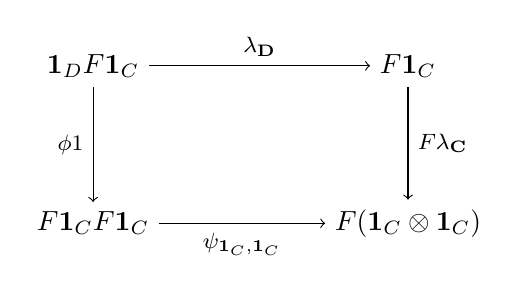
\begin{tikzpicture}
                \node (1) at (0, 0) {$\mathbf{1}_D\circledast F\mathbf{1}_C$};
                \node (2) at (4, 0) {$F\mathbf{1}_C$};
                \node (3) at (0, -2) {$F\mathbf{1}_C\circledast F\mathbf{1}_C$};
                \node (4) at (4, -2) {$F(\mathbf{1}_C\otimes\mathbf{1}_C)$};
                \draw[->] (1) -- node[above]{\footnotesize$\lambda_{\mathbf{D}}$} (2);
                \draw[->] (3) -- node[below]{\footnotesize$\psi_{\mathbf{1}_C, \mathbf{1}_C}$} (4);
                \draw[->] (1) -- node[left]{\footnotesize$\phi\circledast\mathbbm{1}$} (3);
                \draw[->] (2) -- node[right]{\footnotesize$F\lambda_{\mathbf{C}}$} (4);
            \end{tikzpicture}
            \caption{Canonical unit isomorphism.}
            \label{fig:canonical_monoidal_isom}
        \end{figure}
    \end{property}

    \newdef{Lax monoidal functor}{\index{lax!monoidal functor}
        A monoidal functor for which the coherence maps are merely morphisms and not isomorphisms.
    }

    \newdef{Monoidal natural transformation}{
        A natural transformation $\eta$ between (lax) monoidal functors $(F, \psi, \phi_F)$ and $(G, \widetilde{\psi}, \phi_G)$ is said to be (lax) monoidal if it makes the diagrams in figure \ref{fig:monoidal_natural_transformation} commute.
        \begin{figure}[ht!]
            \centering
            \begin{subfigure}[b]{0.49\textwidth}
                \centering
                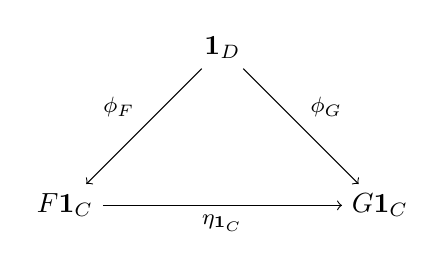
\begin{tikzpicture}
                    \node (1) at (0, 0) {$\mathbf{1}_D$};
                    \node (2) at (-2, -2) {$F\mathbf{1}_C$};
                    \node (3) at (2, -2) {$G\mathbf{1}_C$};
                    \draw[->] (1) -- node[above left]{\footnotesize$\phi_F$} (2);
                    \draw[->] (1) -- node[above right]{\footnotesize$\phi_G$} (3);
                    \draw[->] (2) -- node[below]{\footnotesize$\eta_{\mathbf{1}_C}$} (3);
                \end{tikzpicture}
            \end{subfigure}
            \begin{subfigure}[b]{0.49\textwidth}
                \centering
                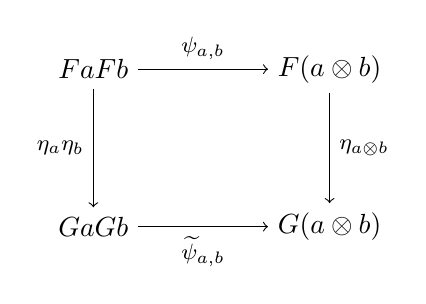
\begin{tikzpicture}
                    \node (1) at (0, 0) {$Fa\circledast Fb$};
                    \node (2) at (3, 0) {$F(a\otimes b)$};
                    \node (3) at (0, -2) {$Ga\circledast Gb$};
                    \node (4) at (3, -2) {$G(a\otimes b)$};
                    \draw[->] (1) -- node[above]{\footnotesize$\psi_{a, b}$} (2);
                    \draw[->] (3) -- node[below]{\footnotesize$\widetilde{\psi}_{a, b}$} (4);
                    \draw[->] (1) -- node[left]{\footnotesize$\eta_a\circledast\eta_b$} (3);
                    \draw[->] (2) -- node[right]{\footnotesize$\eta_{a\otimes b}$} (4);
                \end{tikzpicture}
            \end{subfigure}
            \caption{Monoidal natural transformation.}
            \label{fig:monoidal_natural_transformation}
        \end{figure}
    }

    \newdef{Monoidal equivalence}{\index{monoidal!equivalence}
        Two monoidal categories $\mathbf{C}, \mathbf{D}$ are monoidally equivalent if there exist monoidal functors $\func{F}{C}{D}$ and $\func{G}{D}{C}$ such that there exist monoidal natural isomorphisms $\eta:\mathbbm{1}_C\Rightarrow G\circ F$ and $\varepsilon:F\circ G\Rightarrow\mathbbm{1}_D$.
    }

    \begin{theorem}[MacLane strictness theorem]\index{MacLane!strictness theorem}
        Every monoidal category is monoidally equivalent to a strict monoidal category.
    \end{theorem}

\section{Enriched category theory}\label{section:enriched_category_theory}

    \newdef{Cosmos}{\index{cosmos}
        A complete and cocomplete closed symmetric monoidal category.
    }

    \newdef{Enriched category}{\index{category!enriched}
            Let $(\mathcal{V}, \otimes, \mathbf{1})$ be a monoidal category. A $\mathcal{V}$-enriched category, also called a $\mathcal{V}$-category\footnote{Not to be confused with the notation for fibre categories.}, consists of the following elements:
            \begin{enumerate}
                \item a collection of objects $\ob{C}$;
                \item for every pair of objects $a,b\in\ob{C}$ there is an object $\mathbf{C}(a, b)\in\ob{\mathcal{V}}$ for which the following morphisms exist:
                \begin{itemize}
                    \item $\text{id}_a: \mathbf{1}\rightarrow\mathbf{C}(a, a)$ giving the (enriched) identity morphism;
                    \item $\circ_{abc}:\mathbf{C}(b, c)\otimes\mathbf{C}(a, b)\rightarrow\mathbf{C}(a, c)$ replacing the usual composition.
                \end{itemize}
            \end{enumerate}
            The associativity and unity properties are given by commutative diagrams for the $\text{id}$ and $\circ$ morphisms together with the associators and unitors in $\mathcal{V}$.
    }
    \newdef{Underlying category}{
        Given a $\mathcal{V}$-enriched category $\mathbf{C}$ one defines the underlying category $\mathbf{C}_0$ as follows:
        \begin{itemize}
            \item $\ob{C_0}:=\ob{C}$;
            \item $\mathbf{C}_0(x, y):=\mathcal{V}(\mathbf{1}, \mathbf{C}(x, y))$
        \end{itemize}
        where $\mathbf{1}$ is the monoidal unit in $\mathcal{V}$.
    }
    \begin{property}[$\mathcal{V}$ as a $\mathcal{V}$-category]
        Consider a closed monoidal category $\mathcal{V}$. This category can be given the structure $\widetilde{\mathcal{V}}$ of a $\mathcal{V}$-category by taking the hom-objects to be the internal homs, i.e. $\widetilde{\mathcal{V}}(x, y) := [x, y]$ for all $x,y\in\mathcal{V}$. Property $\ref{cat:internal_hom_property}$ then implies that there exists an isomorphism between the underlying category $\widetilde{\mathcal{V}}_0$ and the original category $\mathcal{V}$.
    \end{property}

    Given two $\mathcal{V}$-enriched categories one can define suitable functors between them:
    \newdef{Enriched functor}{
        A $\mathcal{V}$-enriched functor $\func{F}{C}{D}$ consists of the following data:
        \begin{enumerate}
            \item a function $F_0:\ob{C}\rightarrow\ob{D}$ (as for ordinary functors);
            \item for every two objects $a,b\in\ob{C}$ a morphism $F_{a, b}:\mathbf{C}(a, b)\rightarrow\mathbf{D}(Fa, Fb)$ in $\mathcal{V}$.
        \end{enumerate}
        These have to satisfy the ''obvious'' composition and unit conditions.
    }

    \newdef{Functor tensor product}{\index{tensor!product}\label{cat:functor_tensor_product}
        Consider a covariant functor $\func{G}{C}{M}$ and a contravariant functor $\cfunc{F}{C}{M}$ into a monoidal category $M$. ($\mathbf{C}$ does not have to be enriched over $\mathbf{M}$.) The tensor product of $F$ and $G$ is defined as the following coend:
        \begin{gather}
            F\otimes_{\mathbf{C}} G := \int^{c\in\mathbf{C}}Fc\otimes Gc.
        \end{gather}
    }
    It should be noted that the above tensor product does not produce a new functor, instead it only gives an object in $\mathbf{M}$. A different type of tensor product, one that does give a functor, exists in the enriched setting (however, there is no relation between these two):
    \newdef{Day convolution}{\index{Day convolution}
        Consider a monoidally cocomplete category\footnote{A monoidal category for which the tensor product bifunctor is cocontinuous in each argument.} $\mathbf{M}$ together with a $\mathbf{M}$-enriched category $\mathbf{C}$. Given two $\mathbf{M}$-enriched functors $\func{F,G}{C}{M}$ one defines their tensor product (if it exists) as the following coend:
        \begin{gather}
            F\otimes_{\text{Day}} G := \iint^{x,y\in\mathbf{C}}\mathbf{C}(x\otimes y, -)\otimes Fx\otimes Gy.
        \end{gather}
    }

    \begin{property}[Monoidal structure]
        In the case that $\mathbf{M}$ is a closed symmetric monoidal category the Day convolution is associative and hence defines a monoidal structure on the functor category $[\mathbf{C},\mathbf{M}]$. (The tensor unit is given by the functor (co)represented by the tensor unit in $\mathbf{C}$.)
    \end{property}

    \newdef{Copower}{\index{copower}\index{power} % Both terms are indexed since copowers are rather important on their own.
        Consider a $\mathcal{V}$-enriched category $\mathbf{C}$. One defines the copower (or tensor) functor $\func{\cdot}{\mathcal{V}\times C}{C}$ by the following natural isomorphism:
        \begin{gather}
            \mathbf{C}(v\cdot c, c')\cong[v, \mathbf{C}(c, c')].
        \end{gather}
        Dually, one defines the power (or cotensor) functor $\func{[-,-]}{\mathcal{V}\times C}{C}$ by the following natural isomorphism:
        \begin{gather}
            \mathbf{C}(c, [v, c'])\cong[v, \mathbf{C}(c, c')].
        \end{gather}
        If an enriched category admits all (co)powers then it is also said to be \textbf{(co)powered} (over its enriching category).
    }
    \remark{Equation \ref{cat:internal_symmetry} says that every (closed) symmetric monoidal category $\mathbf{M}$ is powered over itself, the power object just being the internal hom. The same holds for the copower, which is just the tensor product itself.}

    \begin{example}[Disjoint unions]
        Every (co)complete (locally) small category $\mathbf{C}$ admits the structure of a $\mathbf{Set}$-(co)powered category:
        \begin{gather}
            c^S := \prod_{s\in S}c\\
            S\cdot c := \bigsqcup_{s\in S}c.
        \end{gather}
    \end{example}

    The definition and properties of internal hom-functors and (co)powers can be formalized as follows:
    \newdef{Two-variable adjunction}{\index{adjunction}\label{cat:two_variable_adjunction}
        Consider three categories $\mathbf{C, D}$ and $\mathbf{E}$. A two-variable adjunction $\mathbf{C}\times\mathbf{D}\rightarrow\mathbf{E}$ consists of three bifunctors:
        \begin{enumerate}
            \item $\func{-\otimes-}{C\times D}{E}$
            \item $\text{hom}_L:\mathbf{C}^{op}\times\mathbf{E}\rightarrow\mathbf{D}$
            \item $\text{hom}_R:\mathbf{D}^{op}\times\mathbf{E}\rightarrow\mathbf{C}$
        \end{enumerate}
        admitting the following natural isomorphisms:
        \begin{gather}
            \mathbf{E}(c\otimes d, e)\cong\mathbf{C}(c, \text{hom}_L(d, e))\cong\mathbf{D}(d, \text{hom}_R(c, e)).
        \end{gather}
        It should be noted that fixing any of the variables gives rise to ordinary adjunctions in the sense of section \ref{section:category:adjunction}.
    }

    The following definition constructs Kan extensions in the enriched setting, but it can be shown to reduce to \ref{cat:kan_extension} when enriching over $\mathbf{Set}$:
    \newadef{Kan extension}{\index{Kan!extension}\label{cat:enriched_kan_extension}
        Let $\mathbf{C}, \mathbf{D}$ and $\mathbf{E}$ be categories enriched over a monoidal category $\mathcal{V}$. If we assume that $\mathbf{D}$ is copowered over $\mathcal{V}$, then we can define the left Kan extension of $\func{F}{C}{D}$ along $\func{G}{C}{E}$ as the following coend:
        \begin{gather}
            \text{Lan}_GF := \int^{c\in\mathbf{C}}\mathbf{E}(Gc, -)\otimes Fc.
        \end{gather}
        If we assume that $\mathbf{D}$ is powered over $\mathcal{V}$, then we can define the right Kan extension as an end:
        \begin{gather}
            \text{Ran}_GF := \int_{c\in\mathbf{C}}[\mathbf{E}(-, Gc), Fc].
        \end{gather}
    }
    \remark{By choosing $\mathcal{V}=\mathbf{Set}, \mathbf{E}=\mathbf{C}$ and $G=\text{id}_{\mathbf{C}}$ in the previous definition we exactly obtain the ninja Yoneda lemma \ref{cat:ninja_yoneda}.}
    \begin{property}
        Kan extensions computed using (co)ends as above are pointwise in the sense of definition \ref{cat:pointwise_kan_extension}.
    \end{property}

    \newdef{Functor tensor product}{\index{tensor!product}
        Let $\mathbf{D}$ be a category enriched over a monoidal category $\mathcal{V}$. Consider a covariant functor $\func{G}{C}{D}$ and a contravariant functor $\cfunc{F}{C}{\mathcal{V}}$. The tensor product \ref{cat:functor_tensor_product} can be generalized whenever $\mathbf{D}$ is copowered over $\mathcal{V}$:
        \begin{gather}
            \label{cat:copower_product}
            F\otimes_{\mathbf{C}} G := \int^{c\in\mathbf{C}}Fc\cdot Gc.
        \end{gather}
    }

\subsection{Weighted (co)limits}

    We now come back to the definition of ordinary limits and in particular its defining universal property \ref{cat:limit_uproperty}. In this construction the constant functor $\Delta_c$ was one of the main ingredients. This functor can be factorized as $\mathbf{I}\rightarrow1\rightarrow\mathbf{C}$ where $1$ denotes the terminal category. On the level of morphisms this factorization takes the form $\mathbf{I}(i, j)\rightarrow\ast\rightarrow\mathbf{C}(c, c)$ where $\ast$ denotes the terminal one-element set. However, whenever the enriching context is not $\mathbf{Set}$, we do not necessarily have access to a terminal object. Clearly we must change something.

    First we will redefine limits as representing objects. Let us again consider a diagram $\func{D}{I}{C}$. By postcomposition with the Yoneda embedding one obtains the presheaf-valued diagram $\mathbf{C}(-, D-):\mathbf{I}\rightarrow[\mathbf{C}^{op}, \mathbf{Set}]$. Since presheaf categories are complete (example \ref{cat:complete_presheaf_category}), one can always find the limit of this diagram: \[\mathbf{Set}(s, \lim\mathbf{C}(c, D-))\cong\funccat{I}{Set}(\Delta_s, \mathbf{C}(c, D-)).\] If we restrict to the terminal set $s=\ast$, we obtain \[\lim\mathbf{C}(c, D-)\cong\funccat{I}{Set}(\Delta_\ast, \mathbf{C}(c, D-)).\] If this presheaf is representable, we can use the continuity of the covariant hom-functor together with the fact that the Yoneda embedding is fully faithful to show that the representing object is (isomorphic to) $\lim D$, i.e.
    \begin{gather}
        \funccat{I}{Set}(\Delta_\ast, \mathbf{C}(c, D-))\cong\mathbf{C}(c, \lim D).
    \end{gather}

    \newdef{Weighted limit}{\index{limit!weighted}\index{limit!conical}\label{cat:weighted_limit}
        One can now generalize this definition by replacing the constant functor $\Delta_\ast$ by any functor $\func{W}{I}{Set}$. A representing object is then called the $W$-weighted limit of $D$. This object is often denoted by $\wlim{W}D$.\footnote{Another common notation is $\{W, F\}$.} To distinguish weighted limits from ordinary ones, we sometimes call the latter \textbf{conical limits}.
    }

    \begin{remark}
        A motivation for this construction is the following: As was already pointed out in a previous setting, the mere knowledge of global elements $1\rightarrow x$ is often not enough to characterize an object $x$. In general we should look at a collection of generalized elements. When applying this ideology to the case of cones, we see that replacing the functor $\Delta_\ast$ by a more general functor is the same as replacing the global elements $\ast\rightarrow Di$ by generalized elements $Wi\rightarrow Di$.
    \end{remark}

    The generalization to the enriched setting is now evident. There is no reference to the terminal object left and as such we can replace $\mathbf{Set}$ by any enriching category. We will often use (co)end formulas for (weighted) limits, especially in the enriched setting:
    \newformula{Weighted limits}{\index{limit!weighted}\label{cat:weighted_limits}
        By expressing the natural transformations as an end (see equation \ref{cat:natural_end}) and by using the powering in $\mathbf{Set}$ we can express the weighted limit as follows:
        \begin{gather}
            \wlim{W} F \cong \int_{i\in\mathbf{I}}[Wi, Fi].
        \end{gather}
        The generalization to other enriching categories is now straightforward: Consider a diagram $\func{F}{I}{C}$ and a weight functor $\func{W}{I}{\mathcal{V}}$ where $\mathbf{C}$ is $\mathcal{V}$-enriched. If $\mathbf{C}$ is powered over $\mathcal{V}$ then we define the $W$-weighted limit of $F$ by the same formula as before:
        \begin{gather}
            \wlim{W} F := \int_{i\in I}[Wi, Fi].
        \end{gather}
        In a similar way one can define weighted colimits in copowered $\mathcal{V}$-categories as a coend:
        \begin{gather}
            \colim^WF:=\int^{i\in I}Wi\cdot Fi.
        \end{gather}
        Here the weight functor $W$ is required to be contravariant since colimits (and cocones) in general are natural transformations between contravariant functors.
    }

    In the following example we compute the weighted colimit with respect to the Yoneda embedding:
    \begin{example}[Hom-functor]
        Consider a functor $\func{F}{I}{C}$. If we use the Yoneda embedding $\mathcal{Y}c = \mathbf{C}(-, c)$ as weight, we obtain the following property by virtue of the Yoneda lemma:
        \begin{gather}
            \label{cat:weighted_hom_colimit}
            \colim^{\mathcal{Y}c}F\cong Fc.
        \end{gather}
    \end{example}

    We can also express Kan extensions as weighted limits:
    \begin{property}[Kan extensions]
        Consider functors $\func{F}{C}{D}$ and $\func{G}{C}{E}$. If for every $e\in\ob{E}$ the weighted limit $\wlim{\mathbf{E}(e, G-)}F$ exists, then these limits can be combined into a functor which can be shown to be the right Kan extension $\text{Ran}_GF$. The left Kan extension can be obtained through a weighted colimit.
    \end{property}

\section{Internal structures}\index{internal}

    \begin{property}[Eckmann-Hilton]\index{Eckmann-Hilton}\label{category:eckmann_hilton}
        A monoid internal to the category of monoids is the same as a commutative monoid. (See also property \ref{set:eckmann_hilton}.)
    \end{property}

    \newdef{Exponential object}{\index{exponential!object}\label{category:exponential_object}
        In the case of Cartesian (monoidal) categories, i.e. categories where the monoidal structure is given by the (Cartesian) product, the internal hom $\underline{\text{hom}}(a, b)$ is called the exponential object. This is often denoted by $b^a$.
    }
    \newdef{Closed category}{\index{category!closed}
        A (symmetric) monoidal category is said to be closed if it admits all inner homs.
    }

    \newdef{Internal category}{\label{cat:internal_category}
        Let $\mathcal{E}$ be a category with pullbacks. A category $\mathbf{C}$ internal to $\mathcal{E}$ consists of the following objects:
        \begin{enumerate}
            \item an object $C_0\in\ob{\mathcal{E}}$ of objects;
            \item an object $C_1\in\ob{\mathcal{E}}$ of morphisms;
            \item source and target morphisms $s, t\in\mathcal{E}(C_1, C_0)$;
            \item an ''identity-assigning'' morphism $e\in\mathcal{E}(C_0, C_1)$ such that \[s\circ e = \mathbbm{1}_{C_0}\qquad\qquad\qquad t\circ e = \mathbbm{1}_{C_0};\]
            \item a composition morphism $c:C_1\times_{C_0}C_1\rightarrow C_1$ such that the following equations hold:
            \begin{align*}
                s\circ c = s\circ\pi_1\qquad\qquad&\qquad\qquad t\circ c = t\circ\pi_2\\
                \pi_1 = c\circ(e\times_{C_0}\mathbbm{1})\qquad\qquad&\qquad\qquad c\circ(\mathbbm{1}\times_{C_0}e)=\pi_2\\
                c\circ(c\times_{C_0}\mathbbm{1}) &= c\circ(\mathbbm{1}\times_{C_0}c)
            \end{align*}
            where $\pi_1,\pi_2$ are the canonical projections associated with the pullback\footnote{This is the pullback of the pair $(t, s)$.} $C_1\times_{C_0}C_1$.
        \end{enumerate}

        Morphisms between these categories, suitably called \textbf{internal functors}, are given by a pair of morphisms in $\mathcal{E}$, between internal objects and internal morphisms, that preserve composition and identities. Internal natural transformations are defined in a similar way.
    }
    \begin{notation}
        The (bi)category of internal categories in $\mathcal{E}$ is denoted by $\mathbf{Cat}(\mathcal{E})$. It should be noted that for $\mathcal{E}=\mathbf{Set}$ we obtain $\mathbf{Cat}(\mathbf{Set})=\mathbf{Cat}$, i.e. the ordinary (bi)category of small categories.
    \end{notation}
    \begin{adefinition}
        The above definition can be reformulated in a very elegant way: An internal category in $\mathcal{E}$ is a monad in the bicategory $\mathbf{Span}(\mathcal{E})$ (see definition \ref{cat:span_category}).
    \end{adefinition}

    However, functors between internal categories aren't the only relevant morphisms. If we want to define (co)presheafs such as the hom-functor then we stumble upon a problem. In $\mathbf{Cat}$ we had by definition maps to the ambient\footnote{Ordinary category theory has a set-theoretic foundation.} category $\mathbf{Set}$, however for internal categories there does not necessarily exist a morphism $\mathbf{D}\rightarrow\mathcal{E}$. To solve this problem we can consider a more general structure:
    \newdef{Internal diagram}{\index{diagram}
        A left module over a monad in $\mathbf{Span}(\mathcal{E})$. The dual notion is better known as an \textbf{internal presheaf}.
    }
    This is again a specific instance of a more general concept (for more information on the definitions and applications see \cite{maclane, johnstone}):
    \newdef{Internal profunctor}{
        A bimodule between monads in $\mathbf{Span}(\mathcal{E})$.
    }

    \begin{construct}[Internal Yoneda profunctor]
        Consider an internal functor $\func{F}{C}{D}$. This functor induces two internal profunctors $F_*:D\slashedrightarrow C$ and $F^*:C\slashedrightarrow D$. If we expand the definition using spans then we can define these profunctors as follows:

        \qquad For $F_*$ we consider as object map $(F_*)_0:C_0\times_{D_0} D_1:C_0\times D_0$. The action of $f\in D_1$ is given by postcomposition with $f$ in the second factor, while the action of $g\in C_1$ is given by precomposition with $F(g)$ in the second factor (and changing to the domain of $g$ in the first factor).

        It can easily be shown that the profunctors induced by an identity functor $\mathbbm{1}_{\mathbf{C}}$ are isomorphic. In the case of $\mathcal{E}=\mathbf{Set}$ it can be shown that this profunctor is exactly the hom-functor. Therefore we call this in general the (internal) Yoneda profunctor $Y(\mathbf{C})$.
    \end{construct}

\section{Higher category theory}\label{cat:higher_category_theory}
\subsection{\texorpdfstring{$n$-categories}{n-categories}}

    \newdef{$n$-category}{\index{n-category}
        A (strict) $n$-category consists of:
        \begin{itemize}
            \item objects (0-morphisms)
            \item 1-morphisms going between 0-morphisms
            \item ...
            \item $n$-morphisms going between $(n-1)$-morphisms
        \end{itemize}
        such that the composition of $k$-morphisms ($\forall k\leq n$) is associative and satisfies the unit laws as required in an ordinary category. By generalizing this definition to arbitrary $n$ one can define the notion of an $\infty$-category.
    }
    \sremark{$n$-morphisms are also often called \textbf{$n$-cells}. This makes the relation to topological spaces (and in particular simplicial spaces) more visible.}

    \begin{example}[2-category]
        In a 2-category one can compose 2-morphisms in two different ways:
        \begin{enumerate}
            \item \textbf{Horizontal composition}:
            Consider the 2-morphisms $\alpha:f\Rightarrow g$ and $\beta:f'\Rightarrow g'$ where $f'\circ f, g'\circ g$ are well-defined. These 2-morphisms can be composed as \[\beta\circ\alpha: f'\circ f\Rightarrow g'\circ g.\]
            \item \textbf{Vertical composition}:
            Consider the 2-morphisms $\alpha:f\Rightarrow g$ and $\beta:g\Rightarrow h$ where $f, g$ and $h$ have the same domain and codomain. These 2-morphisms can be composed as \[\beta\cdot\alpha: f\Rightarrow h.\]
        \end{enumerate}
        Furthermore, the horizontal and vertical composition should satisfy an interchange law:
        \begin{gather}
            (\alpha\cdot\beta)\circ(\gamma\cdot\delta) = (\alpha\circ\gamma)\cdot(\beta\circ\delta).
        \end{gather}
    \end{example}
    \newdef{\texorpdfstring{$(n, r)$-category}{(n,r)-Category}}{
        A higher ($\infty$-)category for which:
        \begin{itemize}
            \item All parallel $k$-morphisms with $k>n$ are equivalent (and hence trivial).
            \item All $k$-morphisms with $k>r$ are invertible (or equivalences\footnote{In the fully weak $\infty$-sense.}).
        \end{itemize}
    }

    \begin{example}
        The classical example of a 1-category is $\mathbf{Set}$, the classical example of a 2-category is $\mathbf{Cat}$.
    \end{example}

    \newdef{Weak inverse}{\index{weak!inverse}
        Let $\mathbf{C}$ be a 2-category. A 1-morphism $f:x\rightarrow y$ is weakly invertible if there exists a 1-morphism $g:y\rightarrow x$ and 2-isomorphisms $I:g\circ f\Rightarrow\mathbbm{1}_x, J:f\circ g\Rightarrow\mathbbm{1}_y$.
    }

    \begin{property}[Monoidal categories]\index{monoidal!category}\index{delooping!of monoidal categories}\label{cat:monoidal_or_2}
        Consider a monoidal category\footnote{See definition \ref{category:monoidal_category}.} $(\mathbf{C}, \otimes, \mathbf{1})$. From this monoidal category one can construct the so-called \textbf{delooping} $\mathbf{BC}$, which is a bicategory, in the following way:
        \begin{itemize}
            \item There is a single object $\ast$.
            \item The 1-morphisms in $\mathbf{BC}$ are the objects in $\mathbf{C}$.
            \item The 2-morphisms in $\mathbf{BC}$ are the morphisms in $\mathbf{C}$.
            \item Horizontal composition in $\mathbf{BC}$ is the tensor product in $\mathbf{C}$.
            \item Vertical composition in $\mathbf{BC}$ is composition in $\mathbf{C}$.
        \end{itemize}
        Conversely every 2-category with a single object comes from a monoidal category. Hence the 2-category of (pointed) 2-categories with a single object and the 2-category of monoidal categories are equivalent. (This property and its generalizations are the content of the \textit{delooping hypothesis}.)

        In the same way one can deloop a braided monoidal category twice and find an identification with a one-object tricategory with one 1-morphism. However, this identification is not a trivial one as it makes use of the Eckmann-Hilton argument to identify different monoidal structures on this tricategory. (See also section \ref{section:monoidal_n_cat}.)
    \end{property}

\subsection{\texorpdfstring{$n$-functors}{n-functors}}

    \newdef{2-functor}{\index{pseudofunctor}
        A 2-functor $\mathbf{F}:\mathcal{A}\rightarrow\mathcal{B}$ (often called a \textbf{pseudofunctor}) is a morphism between bicategories. It consists of the following data:
        \begin{itemize}
            \item a function $F:\ob{\mathcal{A}}\rightarrow\ob{\mathcal{B}}$;
            \item for every two objects $x,y\in\ob{\mathcal{A}}$ a functor\footnote{This functor is also often denoted by $F$.} $F_{x,y}:\mathcal{A}(x, y)\rightarrow\mathcal{B}(Fx, Fy)$.
        \end{itemize}
        These operations need to satisfy the following coherence conditions:
        \begin{enumerate}
            \item \textbf{Associator}: For every pair of composable 1-morphisms $f\circ g:x\rightarrow y\rightarrow z$ in $\mathcal{A}$ a 2-isomorphism $\gamma_{f, g}:Ff\circ Fg\Rightarrow F(f\circ g)$ such that for every triple of composable morphisms $f\circ g\circ h$ in $\mathcal{A}$ the following identity holds\footnote{Technically one should also insert the associators of the bicategories $\mathcal{A},\mathcal{B}$ to really make this an equality.}:
            \begin{gather}
                \gamma_{f\circ g, h}\circ(\gamma_{f, g}\cdot\mathbbm{1}_{Fh}) = \gamma_{f, g\circ h}\circ(\mathbbm{1}_{Ff}\cdot\gamma_{g, h}).
            \end{gather}
            \item \textbf{Unitor}: For every object $x\in\ob{\mathcal{A}}$ a 2-isomorphism $\iota_x:\mathbbm{1}_{Fx}\Rightarrow F\mathbbm{1}_x$ such that for every morphism $f:x\rightarrow y$ in $\mathcal{A}$ the following identities hold\footnote{Again one should technically insert the unitors of the bicategories $\mathcal{A},\mathcal{B}$ to make these equalities hold.}:
            \begin{gather}
                \iota_y\cdot\mathbbm{1}_{Ff} = \gamma_{\mathbbm{1}_y, f}\\
                \mathbbm{1}_{Ff}\cdot\iota_x = \gamma_{f, \mathbbm{1}_x}.
            \end{gather}
        \end{enumerate}
    }
    \newdef{Lax natural transformation}{
        Consider two 2-functors $\mathbf{F}, \mathbf{G}$ between 2 bicategories $\mathcal{A}$ and $\mathcal{B}$. A lax natural transformation $\eta:\mathbf{F}\Rightarrow\mathbf{G}$ consists of the following data:
        \begin{itemize}
            \item for every object $a\in\ob{\mathcal{A}}$ a 1-morphism $\eta_a:Fa\rightarrow Ga$;
            \item for every 1-morphism $f:a\rightarrow b$ in $\mathcal{A}$ a 2-morphism $\eta_f:Gf\circ\eta_a\Rightarrow\eta_b\circ Ff$ such that the $\eta_f$ are the components of a natural transformation $(\eta_a)^*\circ G\Rightarrow (\eta_b)_*\circ F$ and such that the assignment $f\mapsto\eta_f$ satisfies the ''obvious'' identity and composition axioms.
        \end{itemize}
    }

    \begin{remark}\index{pseudonatural transformation}
        As usual in the higher category context one can speak of lax 2-functors if the associator and unitors above are merely required to be 2-morphisms and of strict 2-functors if these morphisms are required to be identities. If the natural transformations between morphism categories in the definition of a lax natural transformation are all isomorphisms then we call this a  \textbf{pseudonatural transformation}.
    \end{remark}

    \newdef{Modification}{\index{modification}
        Consider two bicategories $\mathcal{A},\mathcal{B}$, two 2-functors $\func{F,G}{\mathcal{A}}{\mathcal{B}}$ and two parallel (lax) natural transformations $\alpha,\beta:\mathbf{F}\Rightarrow\mathbf{G}$. A modification $\mathfrak{m}:\alpha\Rrightarrow\beta$ maps every object $a\in\ob{\mathcal{A}}$ to a 2-morphism $\mathfrak{m}_a:\alpha_a\Rightarrow\beta_a$ such that $\beta_f\circ(\mathbbm{1}_{Gf}\cdot\mathfrak{m}_a) = (\mathfrak{m}_b\cdot\mathbbm{1}_{Ff})\circ\alpha_f$.
    }

    \newdef{Transfor}{\index{transfor}
        A $k$-transfor\footnote{This name was first introduced by \textit{Crans} in \cite{crans_transfors}. A different name which is sometimes used is \textbf{$(n,k)$-transformation}, but this should not be confused with the natural transformations in the context of $(n, r)$-categories.} between two $n$-categories maps $j$-morphisms in one $n$-category to $(j+k)$-morphisms in the other (in a coherent way).
    }
    \begin{example}\index{perturbation}
        The definitions for operations in bicategories above lead us to the following ''explicit'' expressions for $k$-transfors (for small $k$):
        \begin{itemize}
            \item $k=0$: $n$-functors
            \item $k=1$: ($n$-)natural transformations
            \item $k=2$: modifications
            \item $k=3$: \textbf{perturbations}
        \end{itemize}
    \end{example}

    The following definition generalizes the notion of \textit{essential surjectivity} to higher category theory:
    \newdef{$n$-surjective functor}{\index{surjective}
        An $\infty$-functor $\func{F}{C}{D}$ is said to be $n$-surjective if for any two parallel $(n-1)$-morphisms $e, e'$ in $\mathbf{C}$ and $n$-morphism $f: Fe\rightarrow Fe'$ in $\mathbf{D}$ there exists an $n$-morphism $\tilde{f}$ in $\mathbf{C}$ such that $F\tilde{f}\cong f$.
    }

\section{Groupoids}\label{section:groupoids}

    \newdef{Categorical group}{\index{group!categorical}
        Let $(\mathbf{C}, \otimes, \mathbf{1})$ be a monoidal category. This category is called a categorical group, \textbf{gr-category} or \textbf{weak 2-group}\footnote{See also the end of this section.} if it satisfies the following conditions:
        \begin{itemize}
            \item All morphisms are invertible.
            \item Every object is weakly invertible with respect to the monoidal structure.
        \end{itemize}
        By property \ref{cat:monoidal_or_2} above one can equivalently define a weak 2-group as a 2-category with a single object, weakly invertible 1-morphisms and invertible 2-morphisms.
    }

    \newdef{Groupoid}{\index{groupoid}\label{cat:groupoid}
        \nomenclature[S_Grpd]{$\mathbf{Grpd}$}{Category of groupoids.}
        A (small) groupoid $\mathcal{G}$ is a (small) category in which all morphisms are invertible.
    }

    \begin{example}[Delooping]\index{delooping!of groups}\label{cat:group_delooping}
        Consider a group $G$. Its delooping $\mathbf{B}G$ is defined as the one-object groupoid for which $\mathbf{B}G(\ast,\ast)=G$.
    \end{example}

    \newdef{Core}{\index{core}\label{cat:core}
        Let $\mathbf{C}$ be a (small) category. The core Core$(\mathbf{C})\in\mathbf{Grpd}$ of $\mathbf{C}$ is defined as the maximal subgroupoid of $\mathbf{C}$.
    }

    \newdef{Orbit}{\index{orbit}
        Let $\mathcal{G}$ be a groupoid with $O, M$ respectively the set of objects and morphisms. On $O$ one can define an equivalence $a\sim b$ if there exists a morphism $\phi:a\rightarrow b$. The equivalence classes are called orbits and the set of orbits is denoted by $O/M$.
    }
    \newdef{Transitive component}{\index{transitive!component}
        Let $\mathcal{G}$ be a groupoid with $O, M$ respectively the set of objects and morphisms. Let $s, t$ denote the source and target maps on $M$. Given an orbit $o\in O/M$ one defines the transitive component of $M$ associated to $o$ as $s^{-1}(o)$ or equivalently $t^{-1}(o)$.
    }
    \begin{property}
        Every groupoid is a (disjoint) union of its transitive components.
    \end{property}
    \newdef{Transitive groupoid}{\index{transitive!groupoid}
        A groupoid $\mathcal{G}$ is said to be transitive if for all objects $x, y\in\text{ob}(\mathcal{G})$, where $x\neq y$, the set hom$_{\mathcal{G}}(x, y)$ is not empty.
    }

    \newdef{2-Groupoid}{
        A 2-groupoid is a 2-category in which all 1-morphisms are invertible and every 2-morphisms has a 'vertical' inverse. (The 'horizontal' inverse can be constructed from the other inverses.)
    }
    \newdef{Strict 2-group}{
        A 2-group is defined as a 2-groupoid with only one object. From this it follows that the set of 1-morphisms forms a group and so does the set of 2-morphisms under horizontal composition. The 2-morphisms do not form a group under vertical composition\footnote{Because the sources/targets may not match up.}.
    }

    \newdef{$\infty$-groupoid}{
        A $\infty$-category in which all morphisms are invertible. This is equivalent to a $(\infty, 0)$-category in the language of $(n,r)$-categories.
    }

\section{\difficult{Lawvere theories}}

    \newdef{Lawvere theory}{\index{Lawvere!theory}
        Let $\mathbf{F}$ denote the skeleton of $\mathbf{FinSet}$. A Lawvere theory consists of a small category $\mathbf{L}$ and a strict (finite) product preserving \textit{identity-on-objects} functor $\mathcal{L}:\mathbf{F}^{op}\rightarrow\mathbf{L}$.

        Equivalently a Lawvere theory is a small category $\mathbf{L}$ with a \textbf{generic object} $c_0$ such that every object $c\in\ob{L}$ is a finite power of $c_0$.
    }
    \begin{property}
        \nomenclature[S_Law]{$\mathbf{Law}$}{The category of Lawvere theories.}
        All Lawvere theories $(L, \mathcal{L})$ form a category $\mathbf{Law}$. Morphisms between Lawvere theories are (finite) product preserving functors.
    \end{property}

    \newdef{Model}{
        A model or \textbf{algebra} over a Lawvere theory $T$ is a (finite) product-preserving functor $\func{A}{T}{Set}$.
    }

    ?? COMPLETE ??

\section{\difficult{Operad theory}}
\subsection{Operads}

    \newdef{Plain operad\footnotemark}{\index{operad}\index{arity}
        \footnotetext{Also called a \textbf{non-symmetric operad} or \textbf{non-$\Sigma$ operad}.}
        Let $\mathcal{O} = \{P(n)\}_{n\in\mathbb{N}}$ be a sequence of sets, called \textbf{$n$-ary operations} (where $n$ is called the \textbf{arity}). The collection $\mathcal{O}$ is called a plain operad if it satisfies following axioms:
        \begin{enumerate}
            \item $P(1)$ contains an identity element $\mathbbm{1}$.
            \item For all positive integers $n, k_1, \ldots, k_n$ there exists a composition
            \begin{gather}
                \circ:P(n)\times P(k_1)\times\cdots\times P(k_n)\rightarrow P(k_1+\cdots+k_n):(\psi, \theta_1, \ldots, \theta_n)\mapsto \psi\circ(\theta_1, \ldots, \theta_n)
            \end{gather}
            that satisfies two additional axioms:
            \begin{itemize}
                \item Identity:
                \begin{gather}
                    \theta\circ (\mathbbm{1},\ldots,\mathbbm{1}) = \mathbbm{1}\circ\theta = \theta.
                \end{gather}
                \item Associativity:
                \begin{align}
                    \psi\circ\Big(\theta_1\circ&(\theta_{1, 1}, \ldots, \theta_{1, k_1}), \ldots, \theta_n\circ(\theta_{n, 1}, \ldots, \theta_{n, k_n})\Big)\nonumber\\
                    &= \Big(\psi\circ(\theta_1, \ldots, \theta_n)\Big) \circ (\theta_{1,1}, \ldots, \theta_{1, k_1}, \theta_{2, 1}, \ldots, \theta_{n, k_n}).
                \end{align}
            \end{itemize}
        \end{enumerate}
    }
    \begin{notation}
        If one represents the operad using planar tree diagrams the associativity obtains a nice intuitive form. When combining planar tree diagrams in three layers the associativity axiom says that one can first glue the first two layers together or one can first glue the last two layers together.
    \end{notation}

    \remark{One can define plain operads in any monoidal category. In the same way one can define a symmetric operad in any symmetric monoidal category.}

    \begin{example}\index{endomorphism!operad}
        \nomenclature[S_endop]{$\mathcal{E}$nd}{Endomorphism operad}
        Consider a vector space $V$. For every $n\in\mathbb{N}$ one can define the endomorphism algebra End$(V^{\otimes n}, V)$. The endomorphism operad $\mathcal{E}\text{nd}(V)$ is defined as $\{\text{End}(V^{\otimes n}, V)\}_{n\in\mathbb{N}}$.
    \end{example}

    \newdef{$O$-algebra}{\index{algebra!over an operad}
        An object $X$ is called an algebra over an operad $O$ if there exist morphisms \[O(n)\times X^n\rightarrow X\] for every $n\in\mathbb{N}$ satisfying the usual composition and identity laws. Alternatively this can be rephrased as the existence of a (plain) operad morphism $O(n)\rightarrow\mathcal{E}\text{nd}(X)$.
    }
    \begin{example}[Categorical $O$-algebra]
        An $O$-algebra in the category $\mathbf{Cat}$.
    \end{example}

\subsection{Algebraic topology and homotopy theory}

    \newdef{Stasheff operad}{\index{Stasheff!operad}
        A topological operad $\mathcal{K}$ such that $\mathcal{K}(n)$ is given by the $n^{th}$ Stasheff polytope/associahedron. Composition is given by the inclusion of faces.
    }
    \newdef{$A_\infty$-space}{\index{$A_\infty$-space}\label{cat:A_infinity_space}
        An algebra over the Stasheff operad. This induces the structure of a multiplication which is associative up to coherent homotopy.
    }

    \newdef{Little $k$-cubes operad}{\index{operad!little $k$-cubes}
        A topological operad for which every topological space $\mathcal{P}(n)$ consists of all possible configurations of $n$ embedded $k$-cubes in a (unit) $k$-cube. Composition is given by the obvious way of inserting one unit $k$-cube in one of the smaller embedded $k$-cubes.
    }
    \begin{property}[Recognition principle]\index{recognition principle}
        If a connected topological space $X$ forms an algebra over the little $k$-cubes operad then it is (weakly) homotopy equivalent to the $k$-loop space $\Omega^kY$ of a another pointed topological space $Y$. For $k=1$ one should technically use the Stasheff operad, but one can show that this is related to the little interval operad.
    \end{property}

    ?? COMPLETE ??